\chapter[Resultados]{Resultados}

\section{Apresentação dos Histogramas das imagens selecionadas}

Os Histogramas das 4 imagens selecionadas possuem distribuições de valores de \textit{pixels} consideravelmente distintas entre si, como pode ser visualizado nas Figuras \ref{fig:hist-cairn} a \ref{fig:hist-swan}. Destacam-se os Histogramas das imagens \textit{shutters} e \textit{swan}, Figuras \ref{fig:hist-shutters} e  \ref{fig:hist-swan}, respectivamente, por apresentar: a primeira, uma distribuição ao longo de todos valores de \textit{pixels}, sem pico prevalente; a segunda, em oposição àquela, baixa ou nenhuma distribuição, prevalecendo no valor zero, em conformidade com o que é visto na imagem.

\begin{figure}
    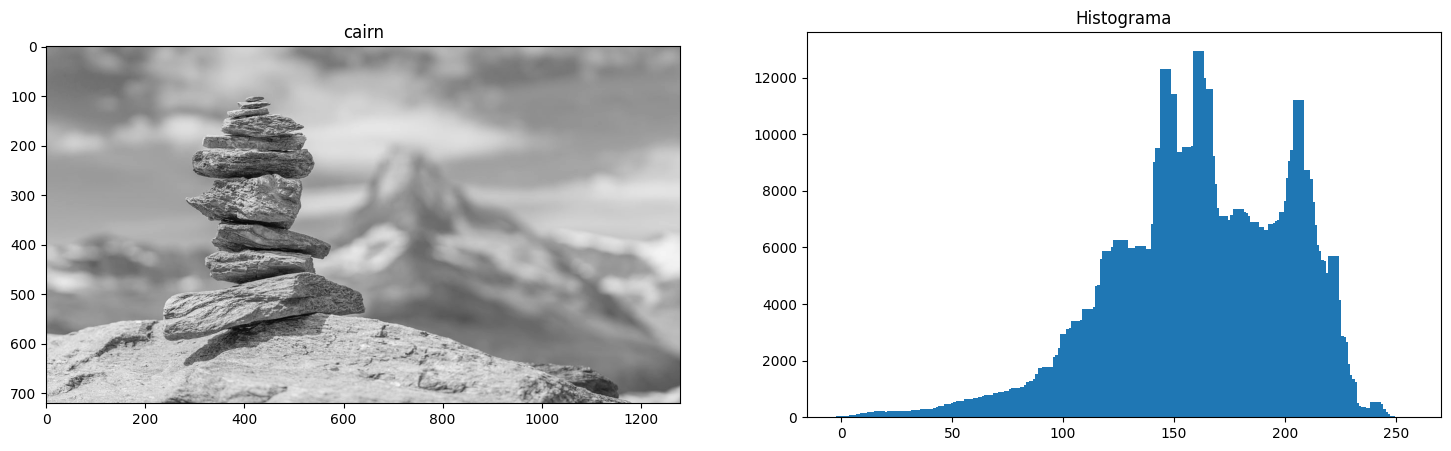
\includegraphics[width=1\linewidth]{Elementos/Figuras/resultados-histograma-cairn.png}
    \caption{Imagem original \textit{cairn} em escala de cinza e o respectivo Histograma}
    \label{fig:hist-cairn}
\end{figure}

\begin{figure}
    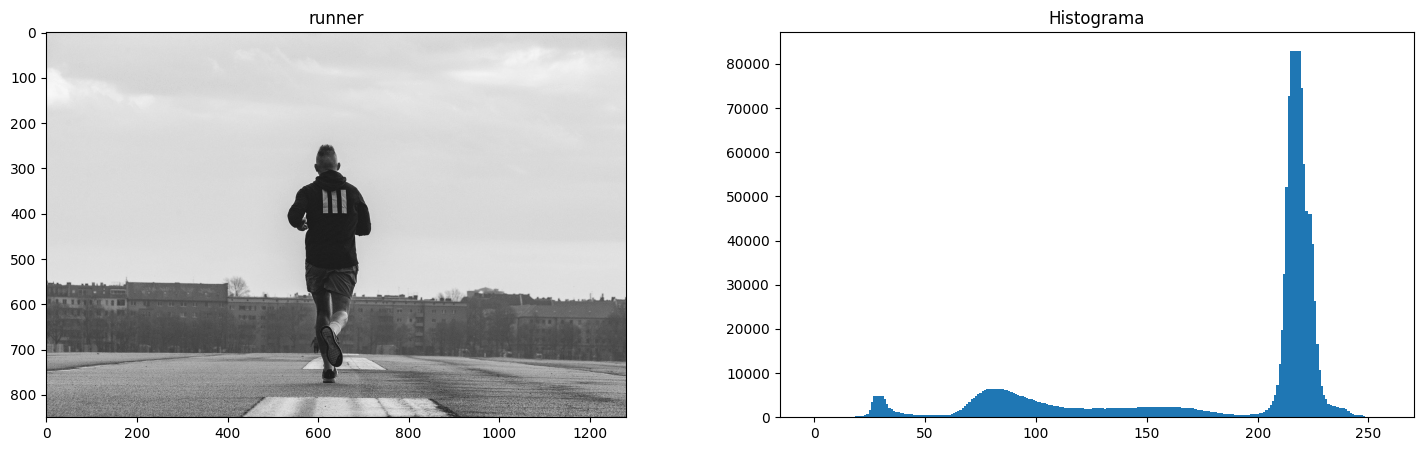
\includegraphics[width=1\linewidth]{Elementos/Figuras/resultados-histograma-runner.png}
    \caption{Imagem original \textit{runner} em escala de cinza e o respectivo Histograma}
    \label{fig:hist-runner}
\end{figure}

\begin{figure}
    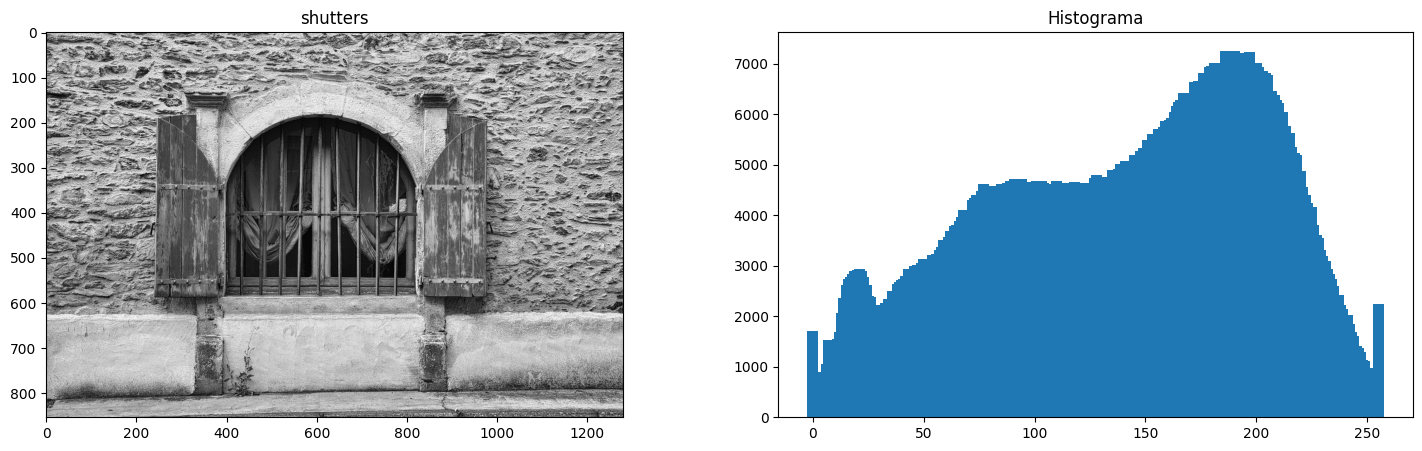
\includegraphics[width=1\linewidth]{Elementos/Figuras/resultados-histograma-shutters.png}
    \caption{Imagem original \textit{shutters} em escala de cinza e o respectivo Histograma}
    \label{fig:hist-shutters}
\end{figure}

\begin{figure}
    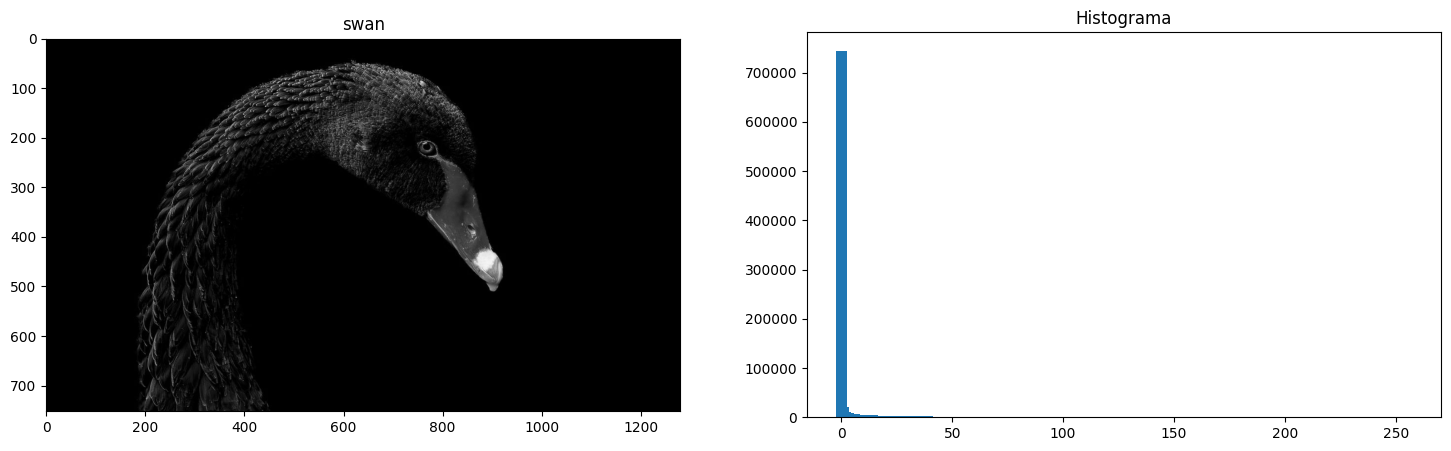
\includegraphics[width=1\linewidth]{Elementos/Figuras/resultados-histograma-swan.png}
    \caption{Imagem original \textit{swan} em escala de cinza e o respectivo Histograma}
    \label{fig:hist-swan}
\end{figure}

% ------------------------------------------------------------- %

\section{Transformação de Intensidade - Correção \textit{gamma}}

Conforme o proposto, foram realizadas duas transformações de intensidade para cada imagem, variando o valor de \textit{gamma} e observados os efeitos que cada aplicação de valor provocou nas imagens. Foram escolhidos: um valor menor que 1 para provocar um deslocamento da distribuição de valores de \textit{pixels} à esquerda, em direção ao zero, resultando em um escurecimento da imagem; e um valor maior que 1 para fazer o deslocamento à direita, em direção ao 255, resultando por conseguinte, em um clareamento da imagem.

As imagens resultantes e seus respectivos Histogramas estão apresentados para visualização e análise nas Figuras \ref{fig:gamma-cairn} a \ref{fig:gamma-swan}. Cada figura contém também a imagem e seu Histograma original para confrontação.

Dos resultados esperados e em conformidade com a transformação realizada, visualiza-se em destaque:

\begin{itemize}
    \item O surgimento de um pico de concentração no escurecimento da imagem \textit{runner} (Figura \ref{fig:gamma-runner});
    \item Na mesma imagem citada no item anterior, no resultado do clareamento, observa-se no Histograma uma separação na distribuição entre os valores de pixel 100 e 150;
    \item Uma forte concentração de valores no escurecimento da imagem \textit{shutters} (Figura \ref{fig:gamma-shutters}), uma vez que originalmente esta imagem possui uma distribuição ao longo de toda a escala de valores;
    \item No escurecimento da imagem \textit{swan} (Figura \ref{fig:gamma-swan}), que originalmente já possui uma concentração predominante em um pico no valor zero, provocou um deslocamento dos poucos valores diferentes de zero, transformando a imagem para quase totalmente zero (preto), fazendo desaparecer a ave objeto da imagem;
    \item Em contrapartida, na mesma imagem citada no item anterior, o clareamento provocou um melhor contorno do objeto da imagem, efeito refletido no respectivo Histograma, através de uma separação observada na distribuição de valores entre os \textit{pixels} de intensidade zero e aproximadamente 30.
\end{itemize}


\begin{figure}
    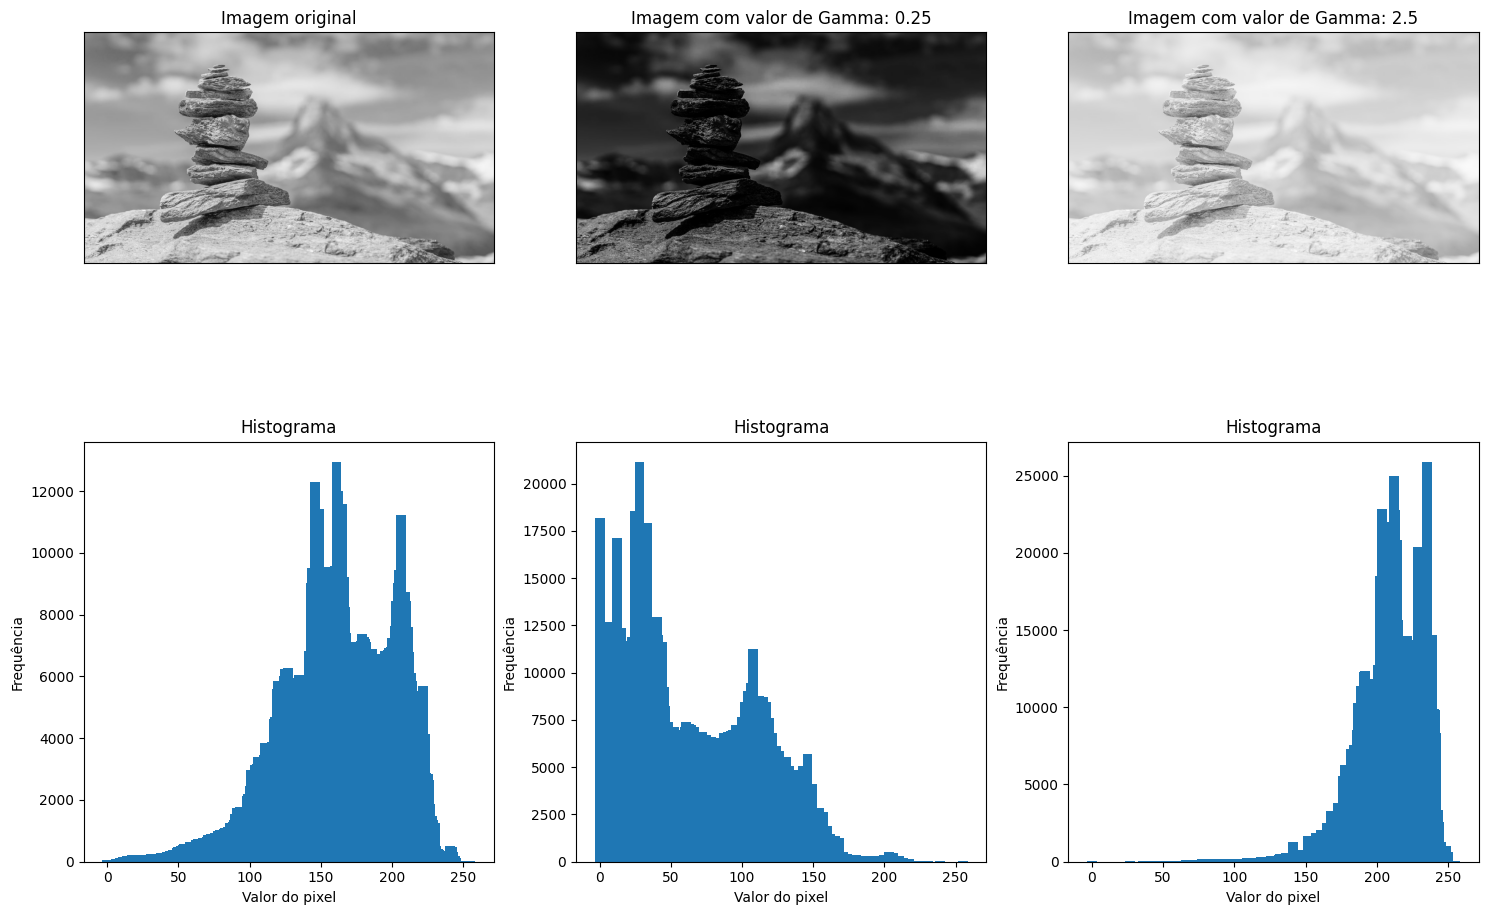
\includegraphics[width=1\linewidth]{Elementos/Figuras/resultados-gamma-cairn.png}
    \caption{Imagem \textit{cairn} em transformação por \textit{Gamma Correction}}
    \label{fig:gamma-cairn}
\end{figure}

\begin{figure}
    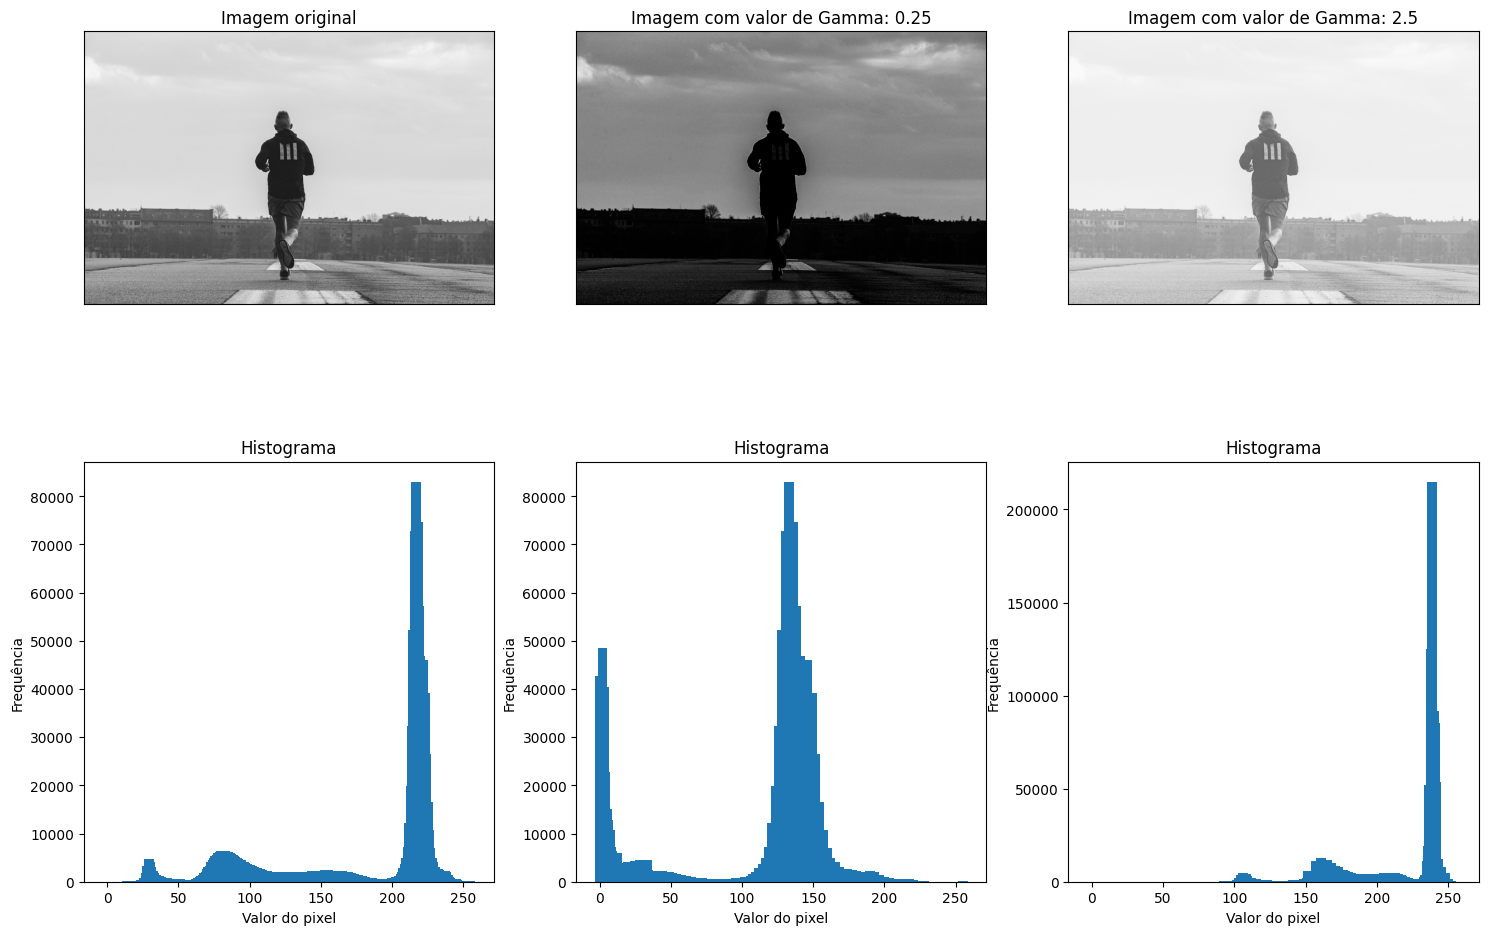
\includegraphics[width=1\linewidth]{Elementos/Figuras/resultados-gamma-runner.png}
    \caption{Imagem \textit{runner} em transformação por \textit{Gamma Correction}}
    \label{fig:gamma-runner}
\end{figure}

\begin{figure}
    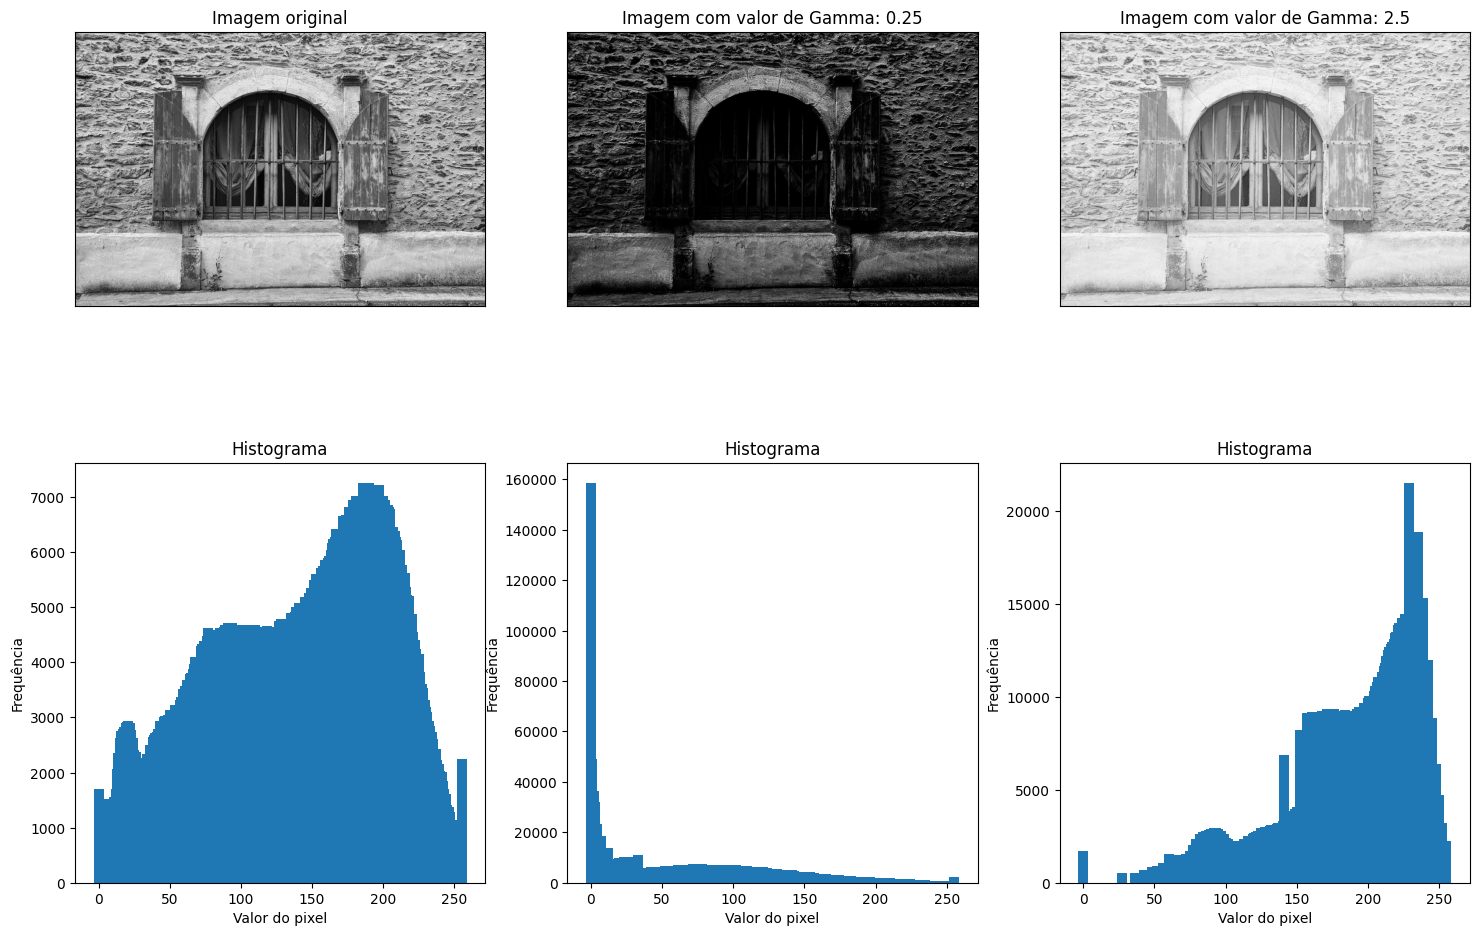
\includegraphics[width=1\linewidth]{Elementos/Figuras/resultados-gamma-shutters.png}
    \caption{Imagem \textit{shutters} em transformação por \textit{Gamma Correction}}
    \label{fig:gamma-shutters}
\end{figure}

\begin{figure}
    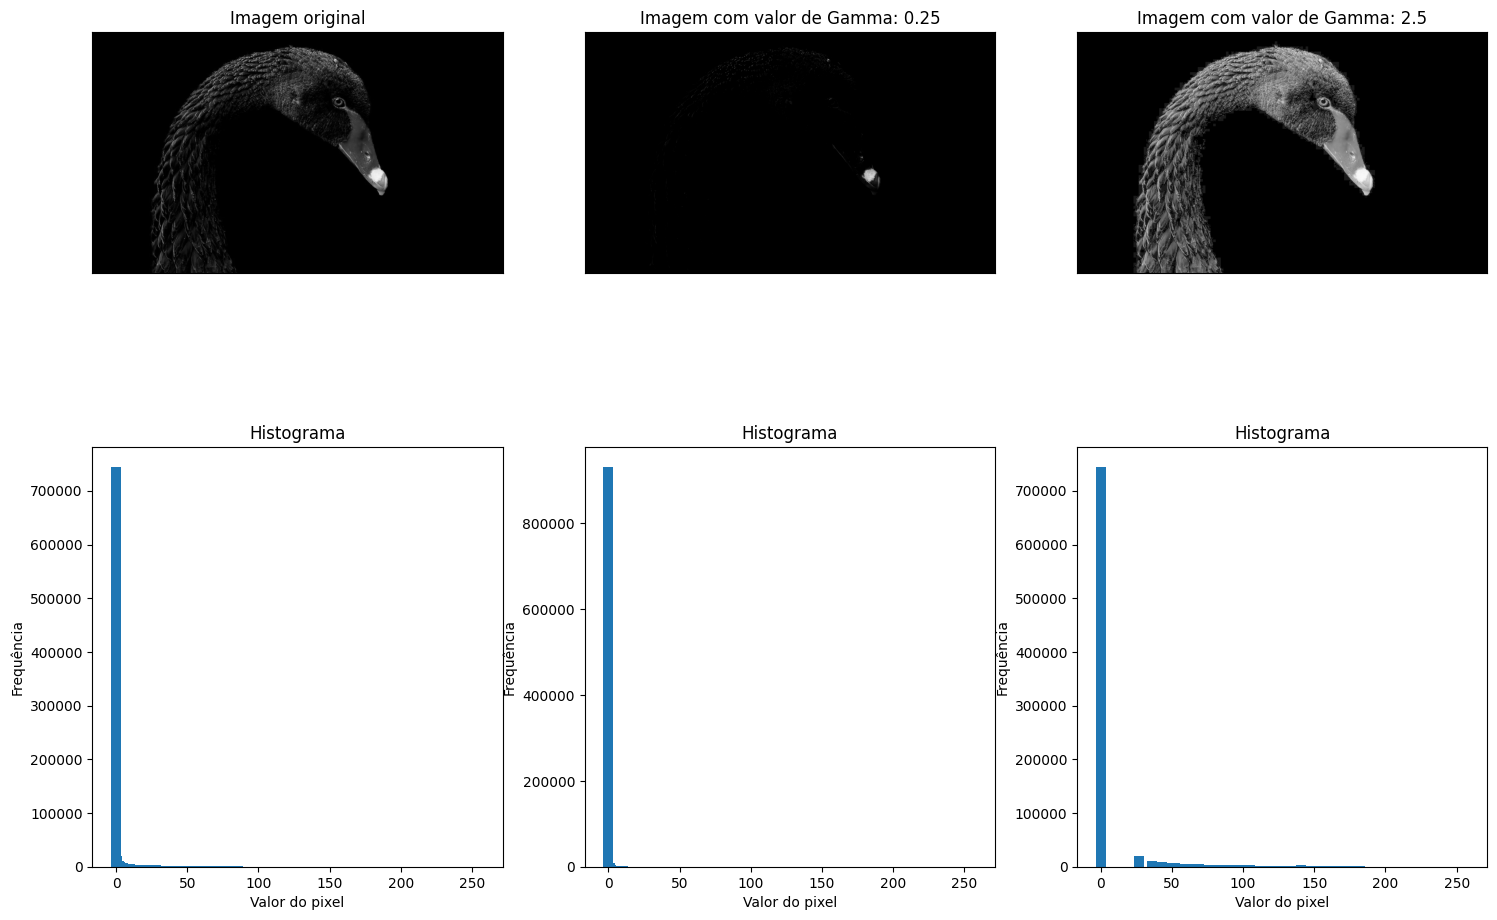
\includegraphics[width=1\linewidth]{Elementos/Figuras/resultados-gamma-swam.png}
    \caption{Imagem \textit{swan} em transformação por \textit{Gamma Correction}}
    \label{fig:gamma-swan}
\end{figure}

% -------------------------------------------------------------- %

\section{Binarização}

A binarização da imagem \textit{cairn} original e com os valores de \textit{gamma} $0.25$ e $2.5$ utilizando o limiar $127$ e o método \textit{Otsu} $157.0$, $67.0$ e $200.0$.
Conforme Figura \ref{fig:binarizacao-cairn}, podemos observar que na redução \textit{gamma} o resultado é uma imagem mais escura quando o valor de \textit{gamma} é $0.25$ e sendo o oposto quando o valor de \textit{gamma} é $2.5$.

\begin{figure}[h!]
    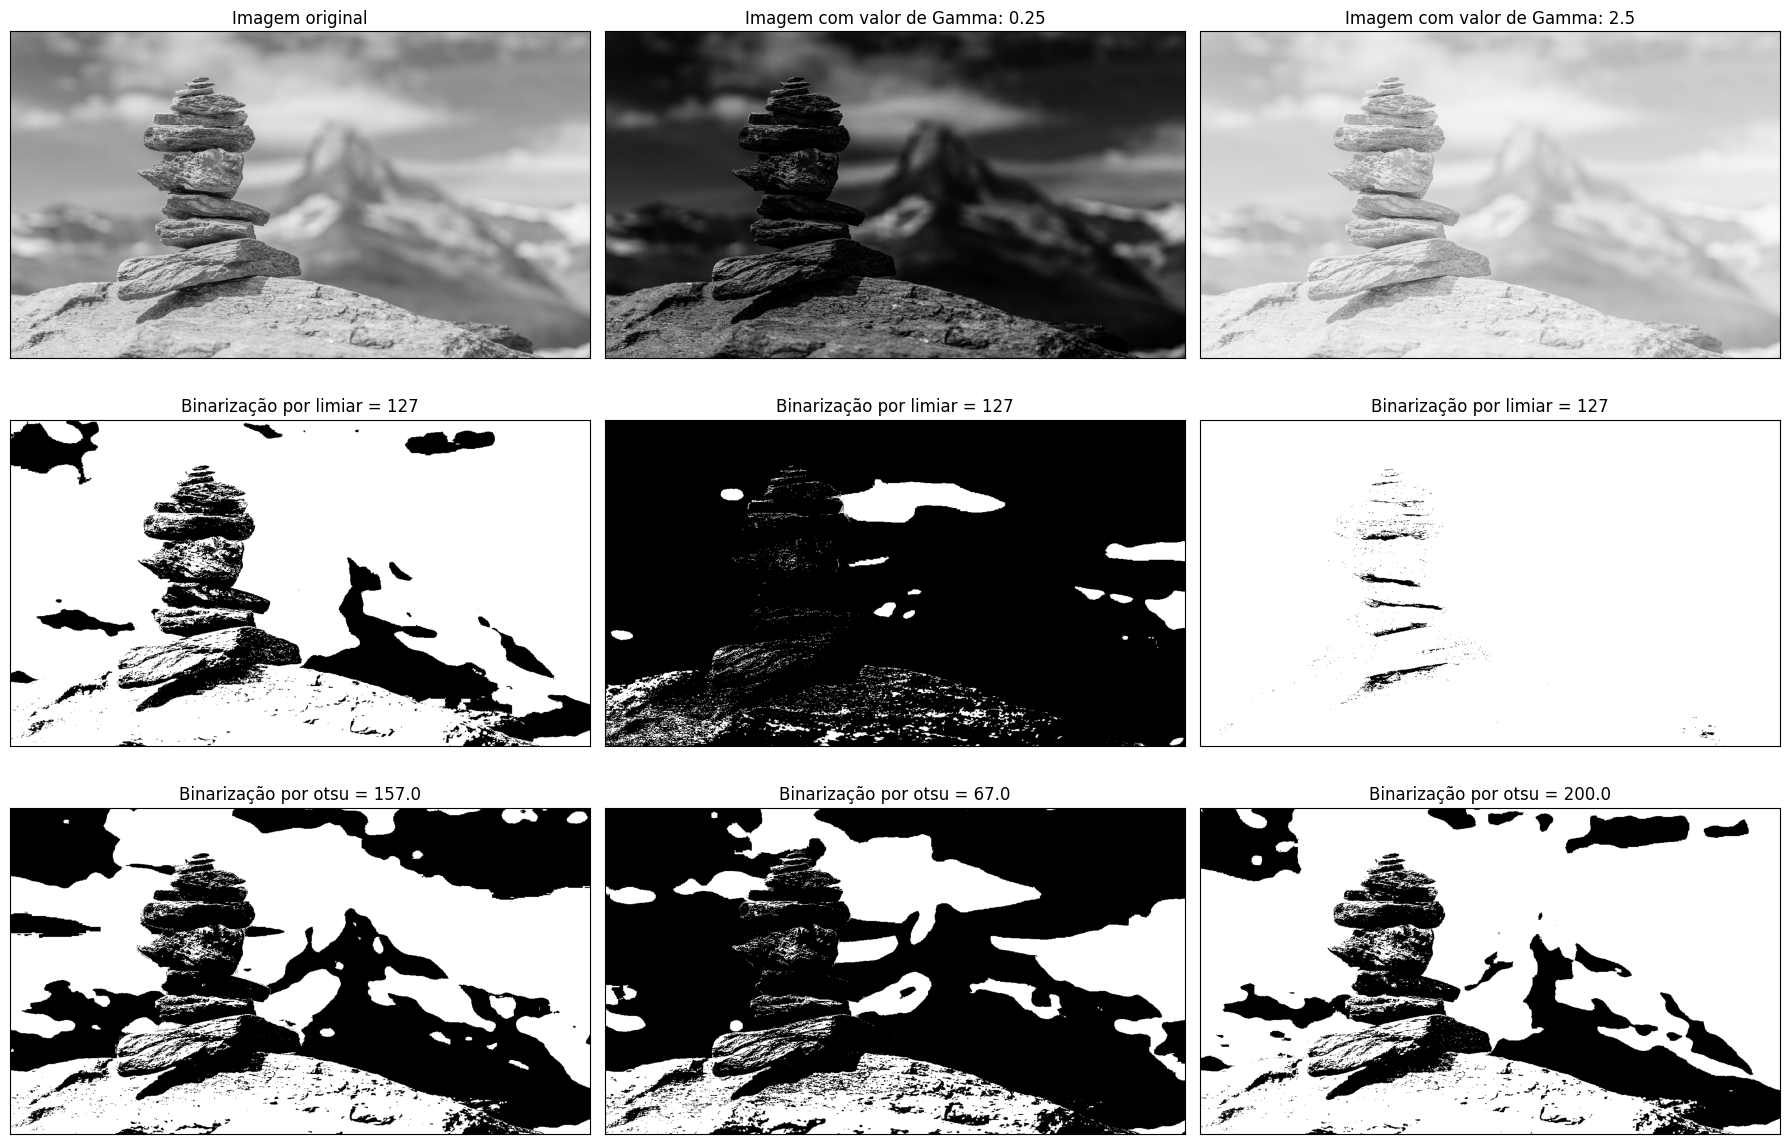
\includegraphics[width=1\linewidth]{Elementos/Figuras/resultados-binarizacao-cairn.png}
    \caption{Imagem \textit{cairn} em transformação por métodos de binarização}
    \label{fig:binarizacao-cairn}
\end{figure}

A binarização da imagem \textit{runner} original e com os valores de \textit{gamma} $0.25$ e $2.5$ utilizando o limiar $127$ e o método \textit{Otsu} $154.0$, $75.0$ e $199.0$.
Conforme Figura \ref{fig:binarizacao-runner}, podemos observar que na redução \textit{gamma} o resultado é uma imagem mais escura quando o valor de \textit{gamma} é $0.25$ e sendo o oposto quando o valor de \textit{gamma} é $2.5$.

\begin{figure}[h!]
    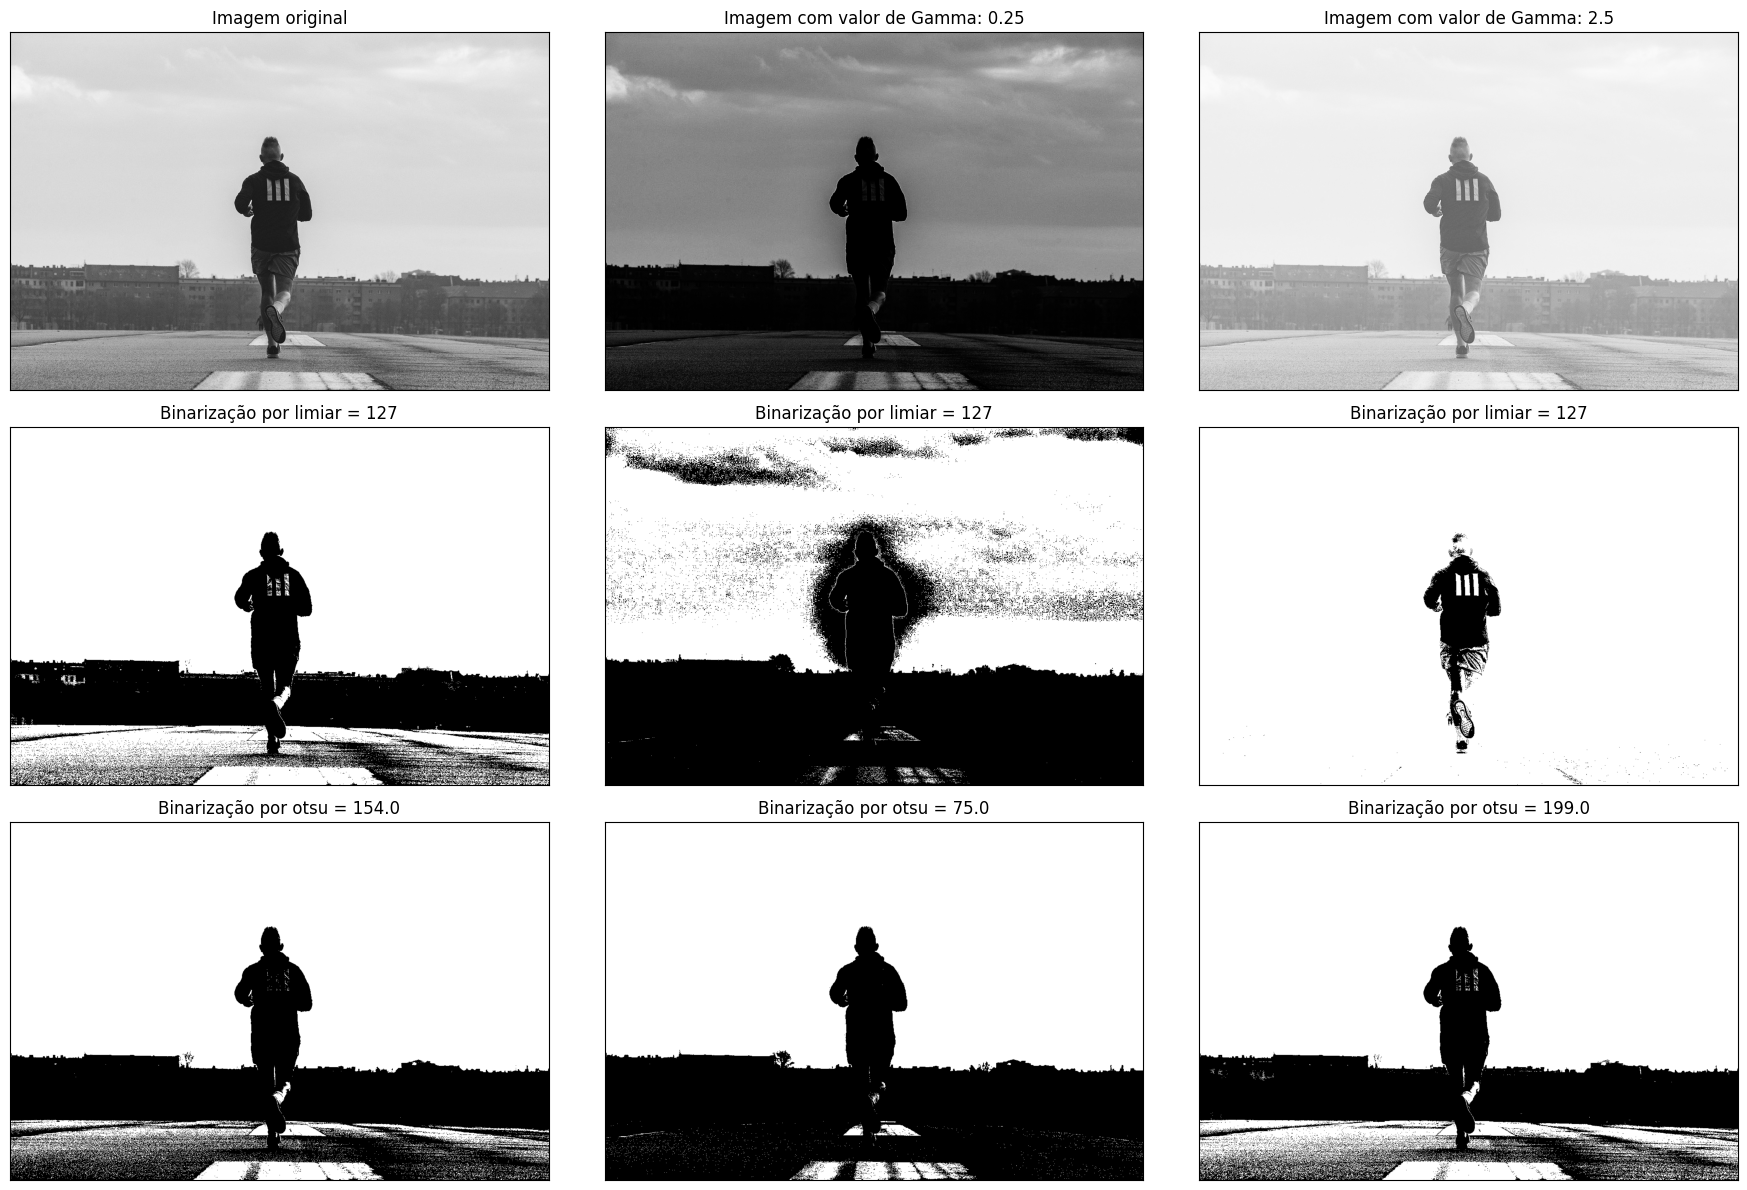
\includegraphics[width=1\linewidth]{Elementos/Figuras/resultados-binarizacao-runner.png}
    \caption{Imagem \textit{runner} em transformação por métodos de binarização}
    \label{fig:binarizacao-runner}
\end{figure}

Temos neste exemplo a imagem \textit{shutters} original e com os valores de \textit{gamma} $0.25$ e $2.5$ utilizando o limiar $127$ e o método \textit{Otsu} $130.0$, $70.0$ e $178.0$.
Conforme Figura \ref{fig:binarizacao-shutters}, observamos que na redução \textit{gamma} o resultado é uma imagem mais escura quando o valor de \textit{gamma} é $0.25$ e sendo o oposto quando o valor de \textit{gamma} é $2.5$.

\begin{figure}[h!]
    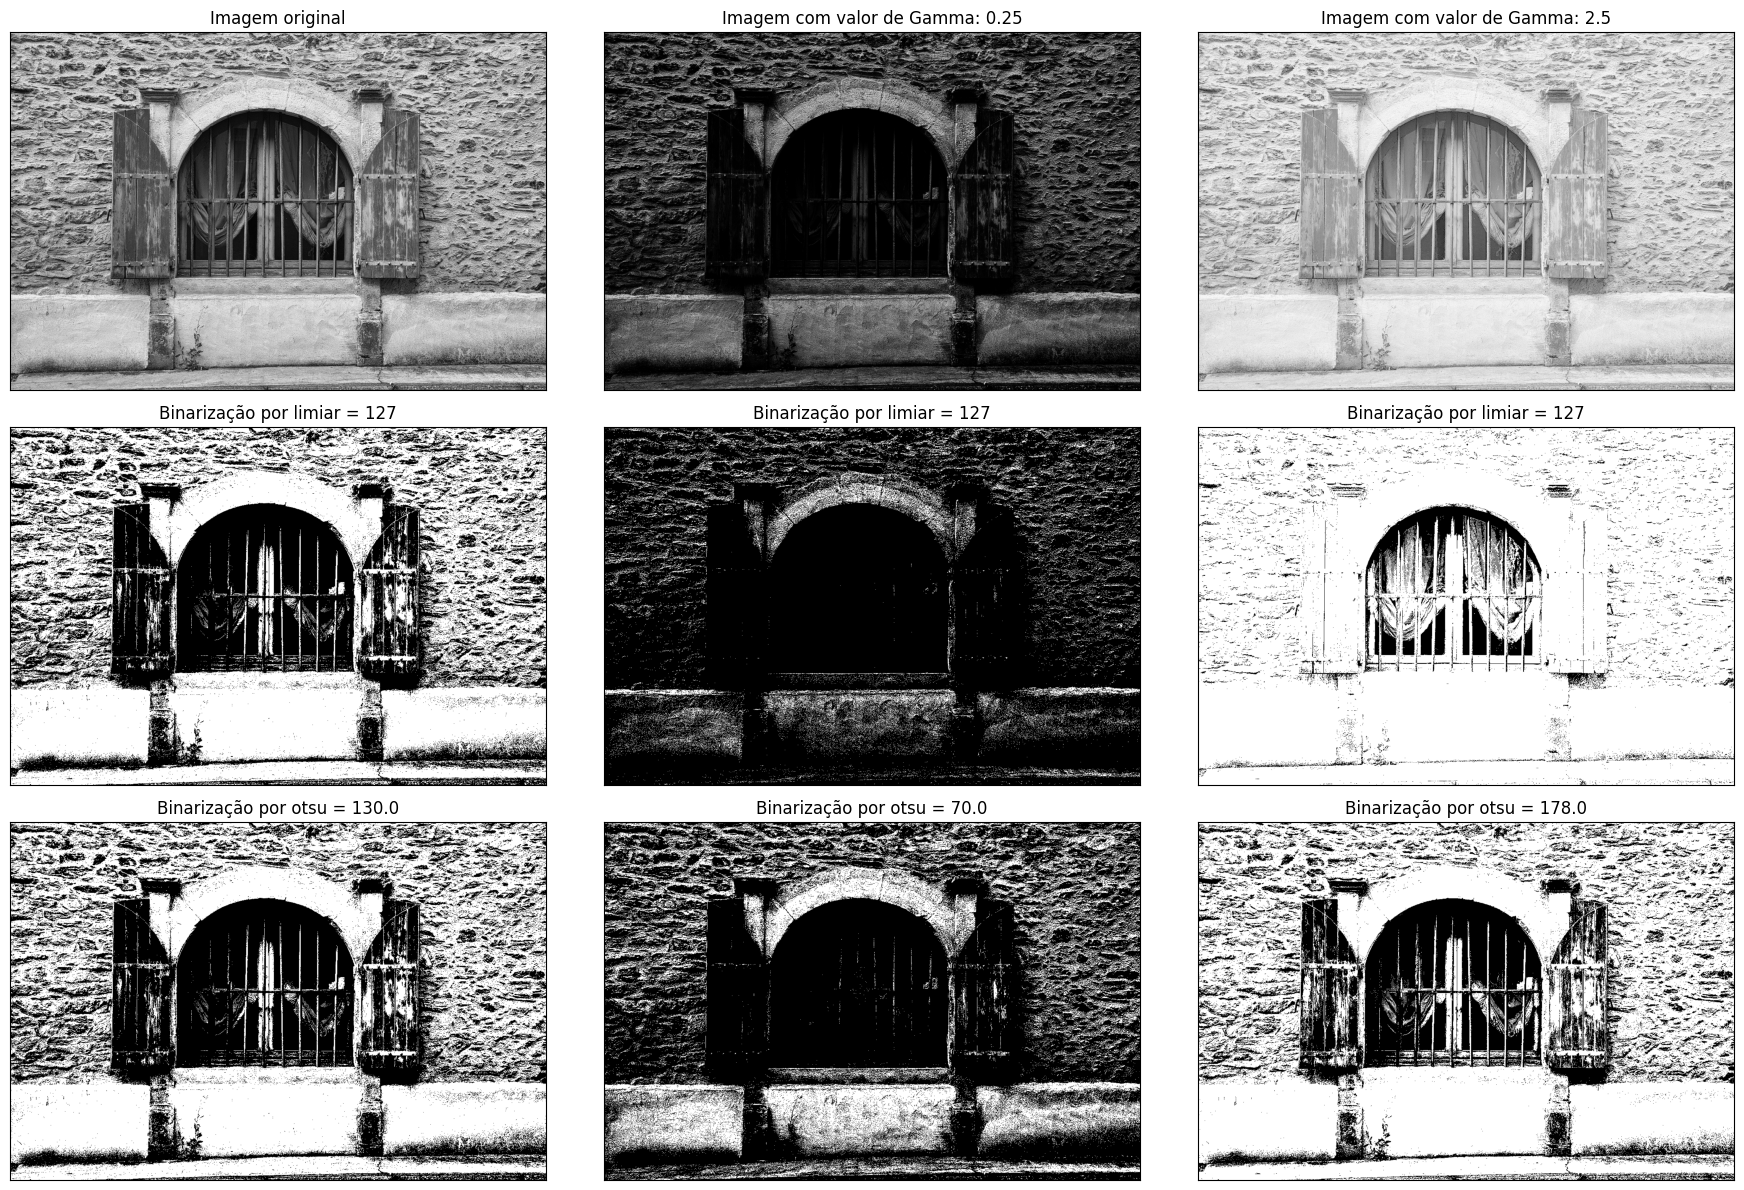
\includegraphics[width=1\linewidth]{Elementos/Figuras/resultados-binarizacao-shutters.png}
    \caption{Imagem \textit{shutters} em transformação por métodos de binarização}
    \label{fig:binarizacao-shutters}
\end{figure}

A binarização da imagem \textit{swan} original e com os valores de \textit{gamma} $0.25$ e $2.5$ utilizando o limiar $127$ e o método \textit{Otsu} $37.0$, $58.0$ e $76.0$.
Conforme Figura \ref{fig:binarizacao-swan}, podemos observar que na redução \textit{gamma} o resultado é uma imagem mais escura quando o valor de \textit{gamma} é $0.25$ e sendo o oposto quando o valor de \textit{gamma} é $2.5$.

\begin{figure}[h!]
    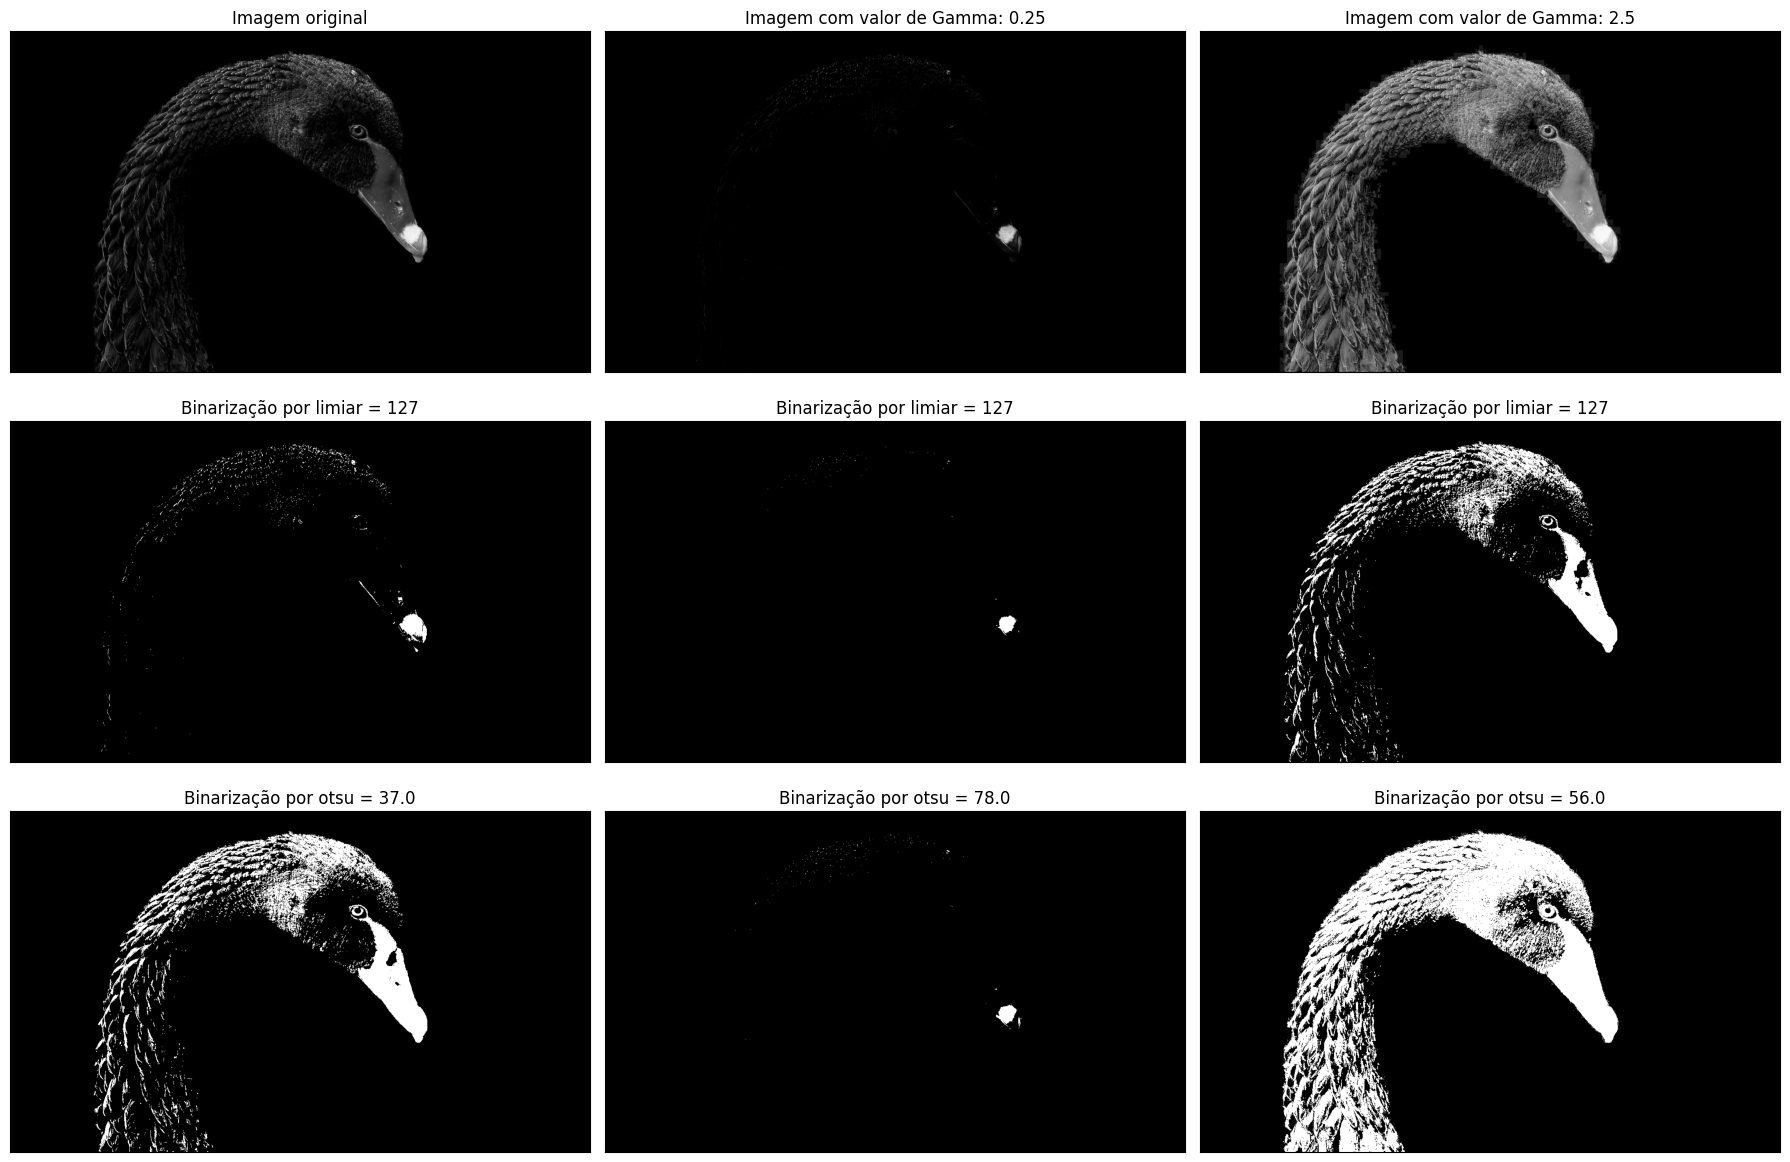
\includegraphics[width=1\linewidth]{Elementos/Figuras/resultados-binarizacao-swan.png}
    \caption{Imagem \textit{swan} em transformação por métodos de binarização}
    \label{fig:binarizacao-swan}
\end{figure}

% -------------------------------------------------------------- %

\section{Modificação de \textit{bits} menos e mais significativos}

Conforme proposto, foram zerados os LSBs e os MSBs das imagens utilizadas nesta atividade a fim de realizar análises acerca da quantidade máxima de \textit{bits} mais e menos significativos que podem ser utilizados para a ocultação de informações.

\subsection{Comparação dos histogramas das imagens com LSBs zerados}

As imagens com 1, 2, 3, 4, 5, 6 e 7 LSBs (Figuras \ref{fig:swan-lsb} a \ref{fig:cairn-lsb})foram dispostas lado a lado.  Ao lado de cada imagem está o seu histograma, por meio do qual pode-se observar a diminuição do número de tonalidades conforme a quantidade de LSBs aumenta. 

\begin{figure}[h!]
    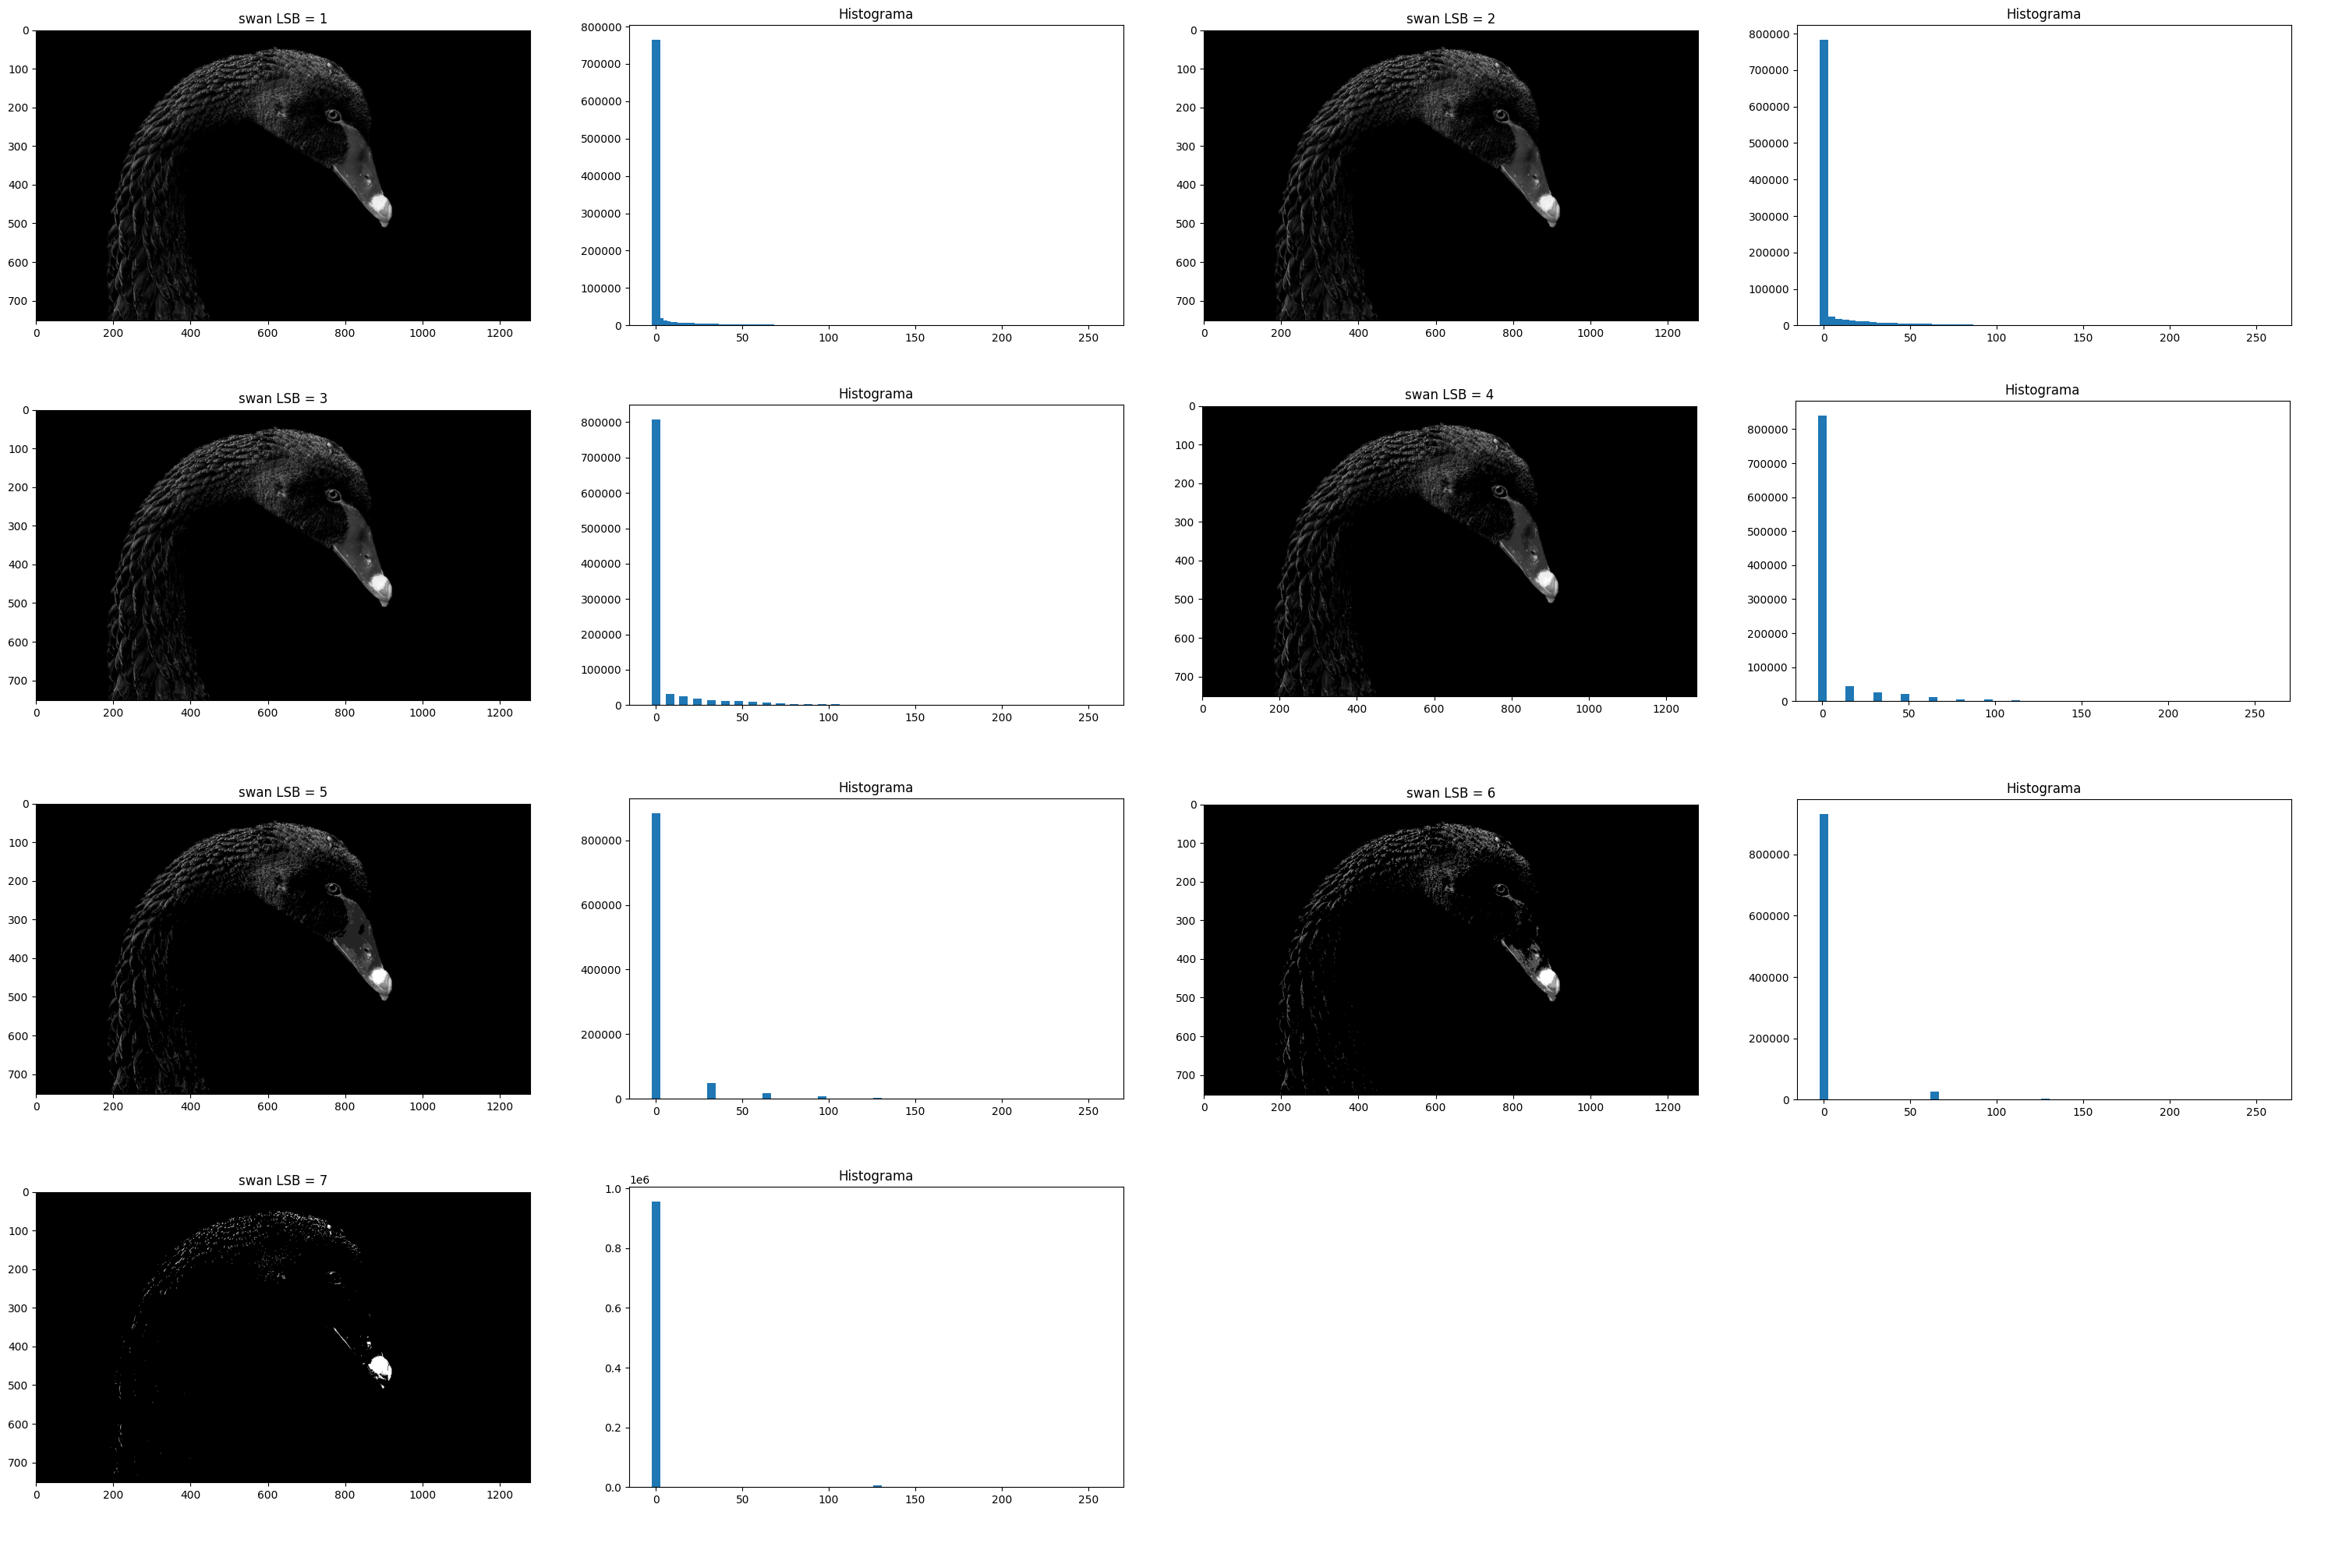
\includegraphics[width=1\linewidth]{Elementos//Figuras/swan_lsb.png}
    \caption{Da esquerda para a direita e de cima para baixo temos: Imagem Swan com 1, 2, 3, 4, 5, 6 e 7 LSBs zerados.}
    \label{fig:swan-lsb}
\end{figure}

Ao observar os histogramas da imagem \textit{swan} (Figura \ref{fig:swan-lsb}), percebe-se que a diminuição da quantidade de tonalidades não é tão notável como nas demais imagens, isso ocorre pois a imagem original não apresenta grande variação em seus níveis de cinza, além de apresentar uma única tonalidade com frequência muito mais alta do que as demais.

\begin{figure}[h!]
    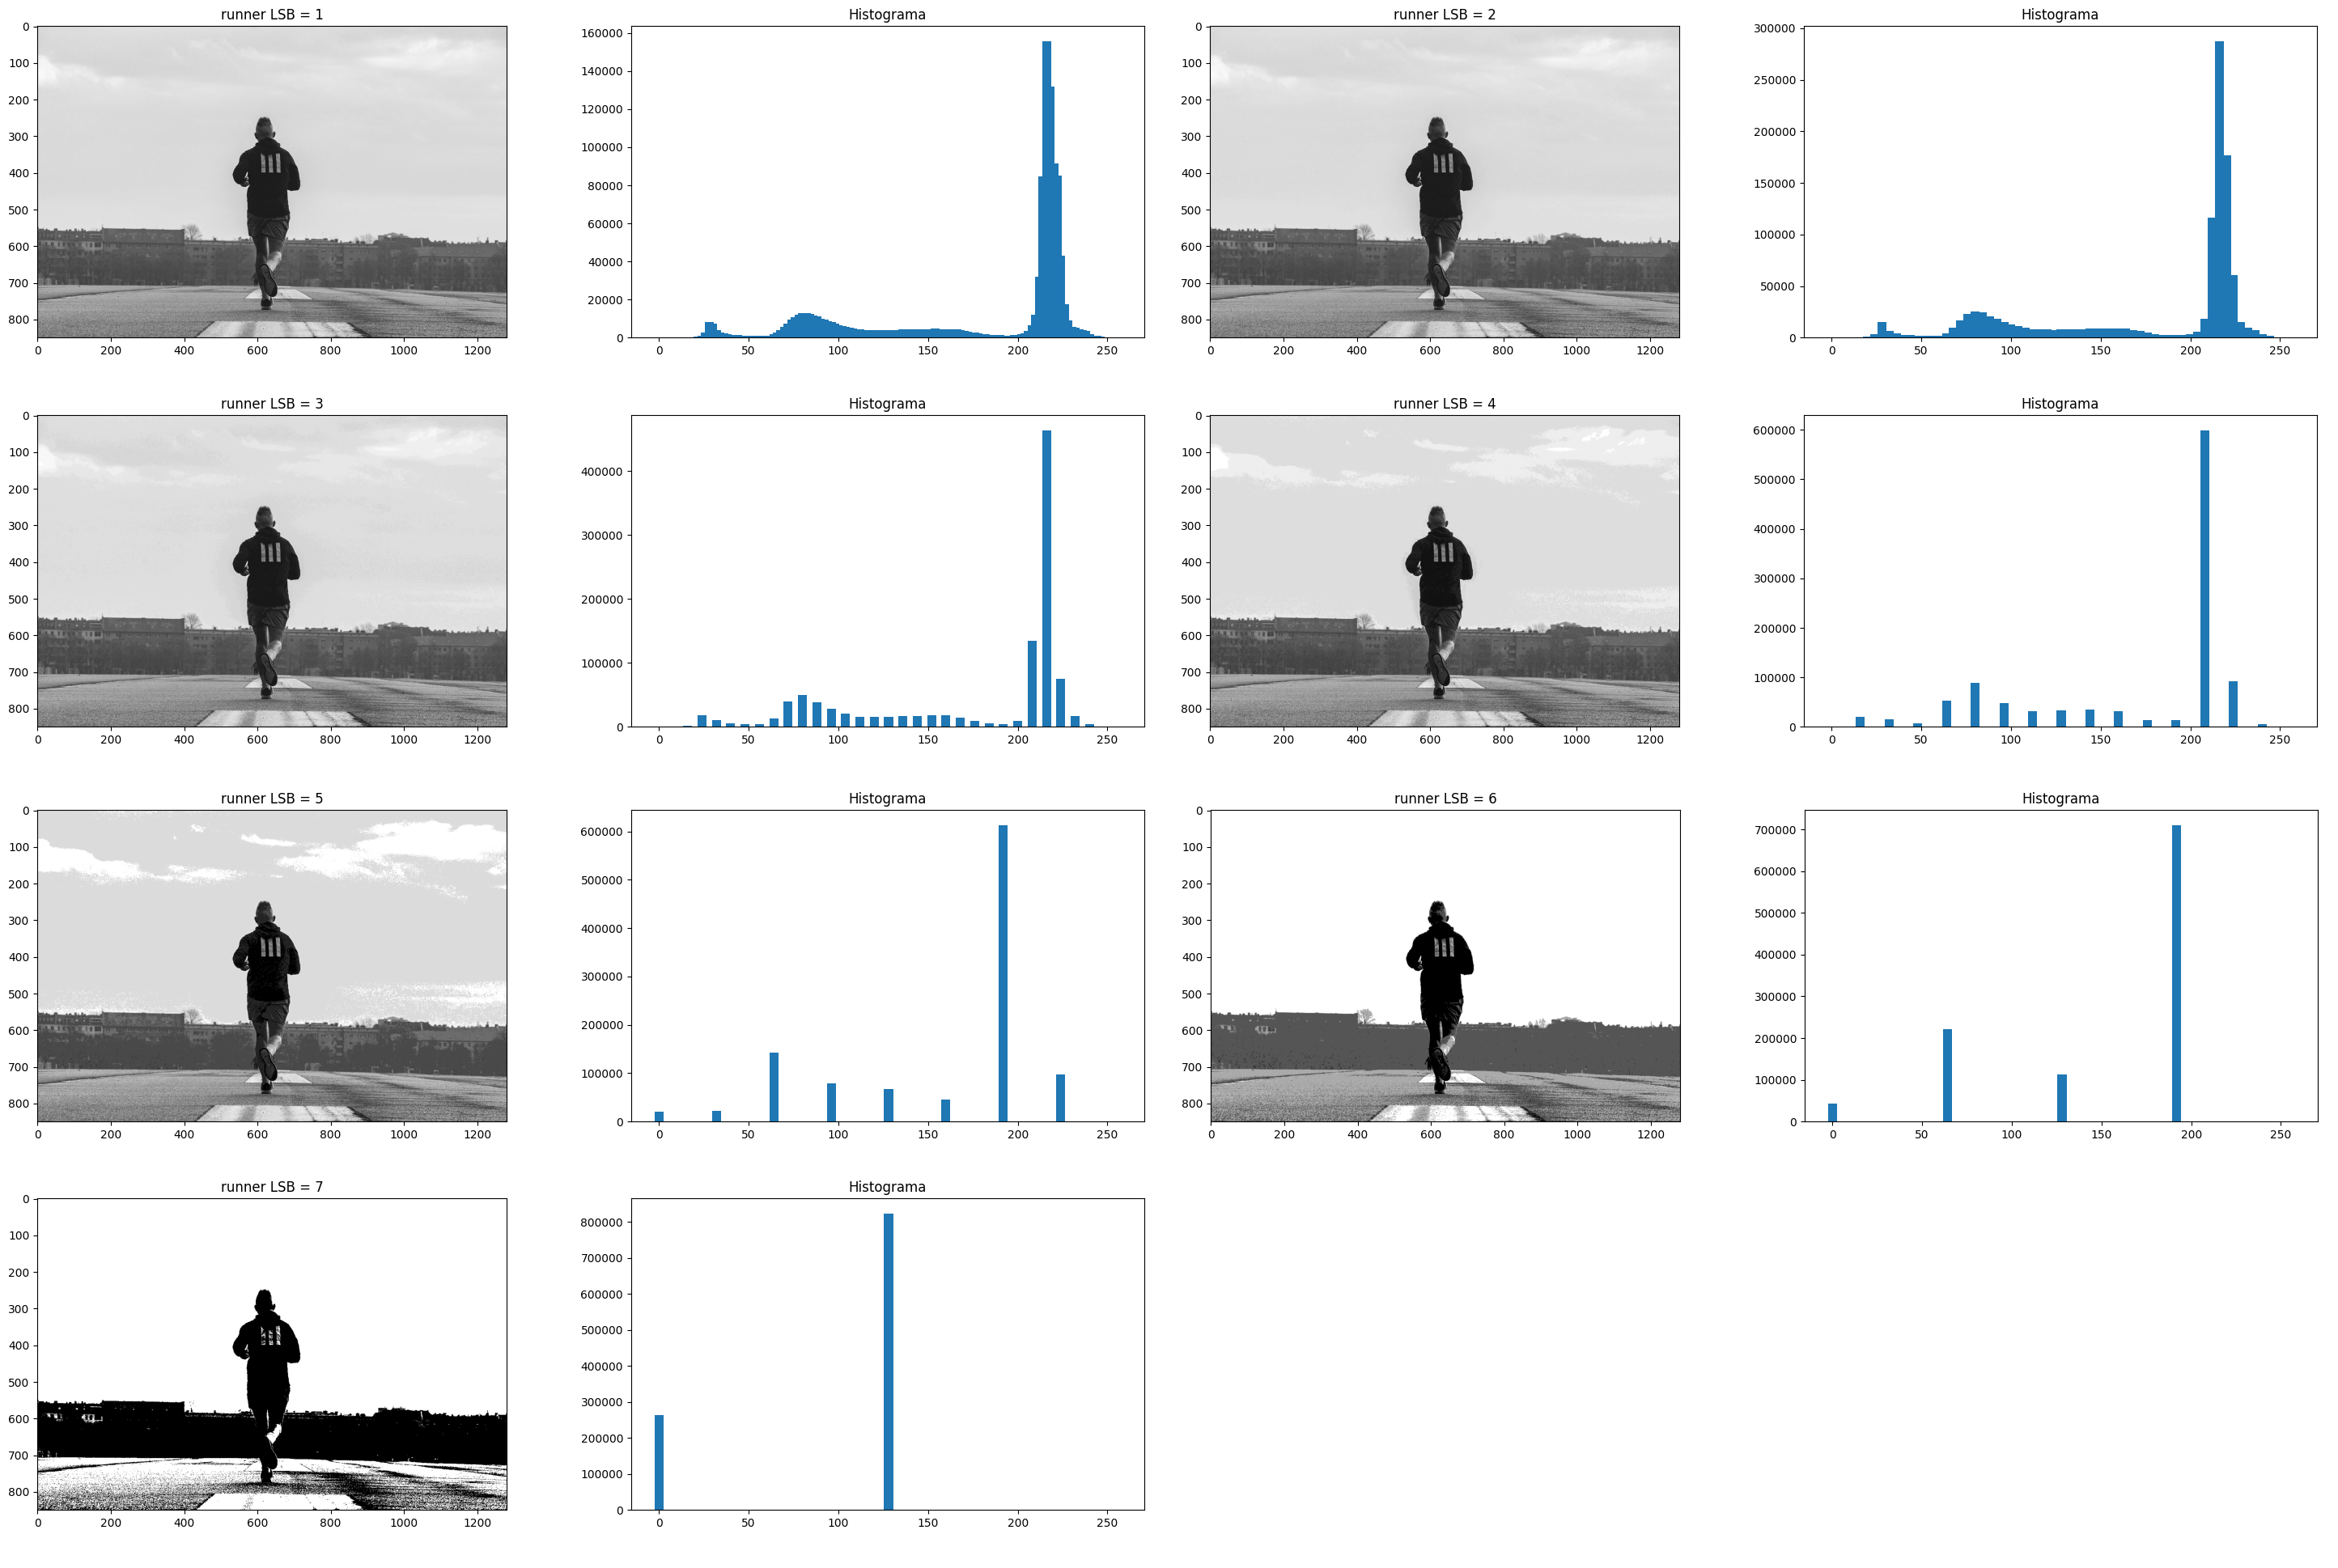
\includegraphics[width=1\linewidth]{Elementos//Figuras/runner_lsb.png}
    \caption{Da esquerda para a direita e de cima para baixo temos: Imagem Runner com 1, 2, 3, 4, 5, 6 e 7 LSBs zerados.}
    \label{fig:runner-lsb}
\end{figure}

\begin{figure}[h!]
    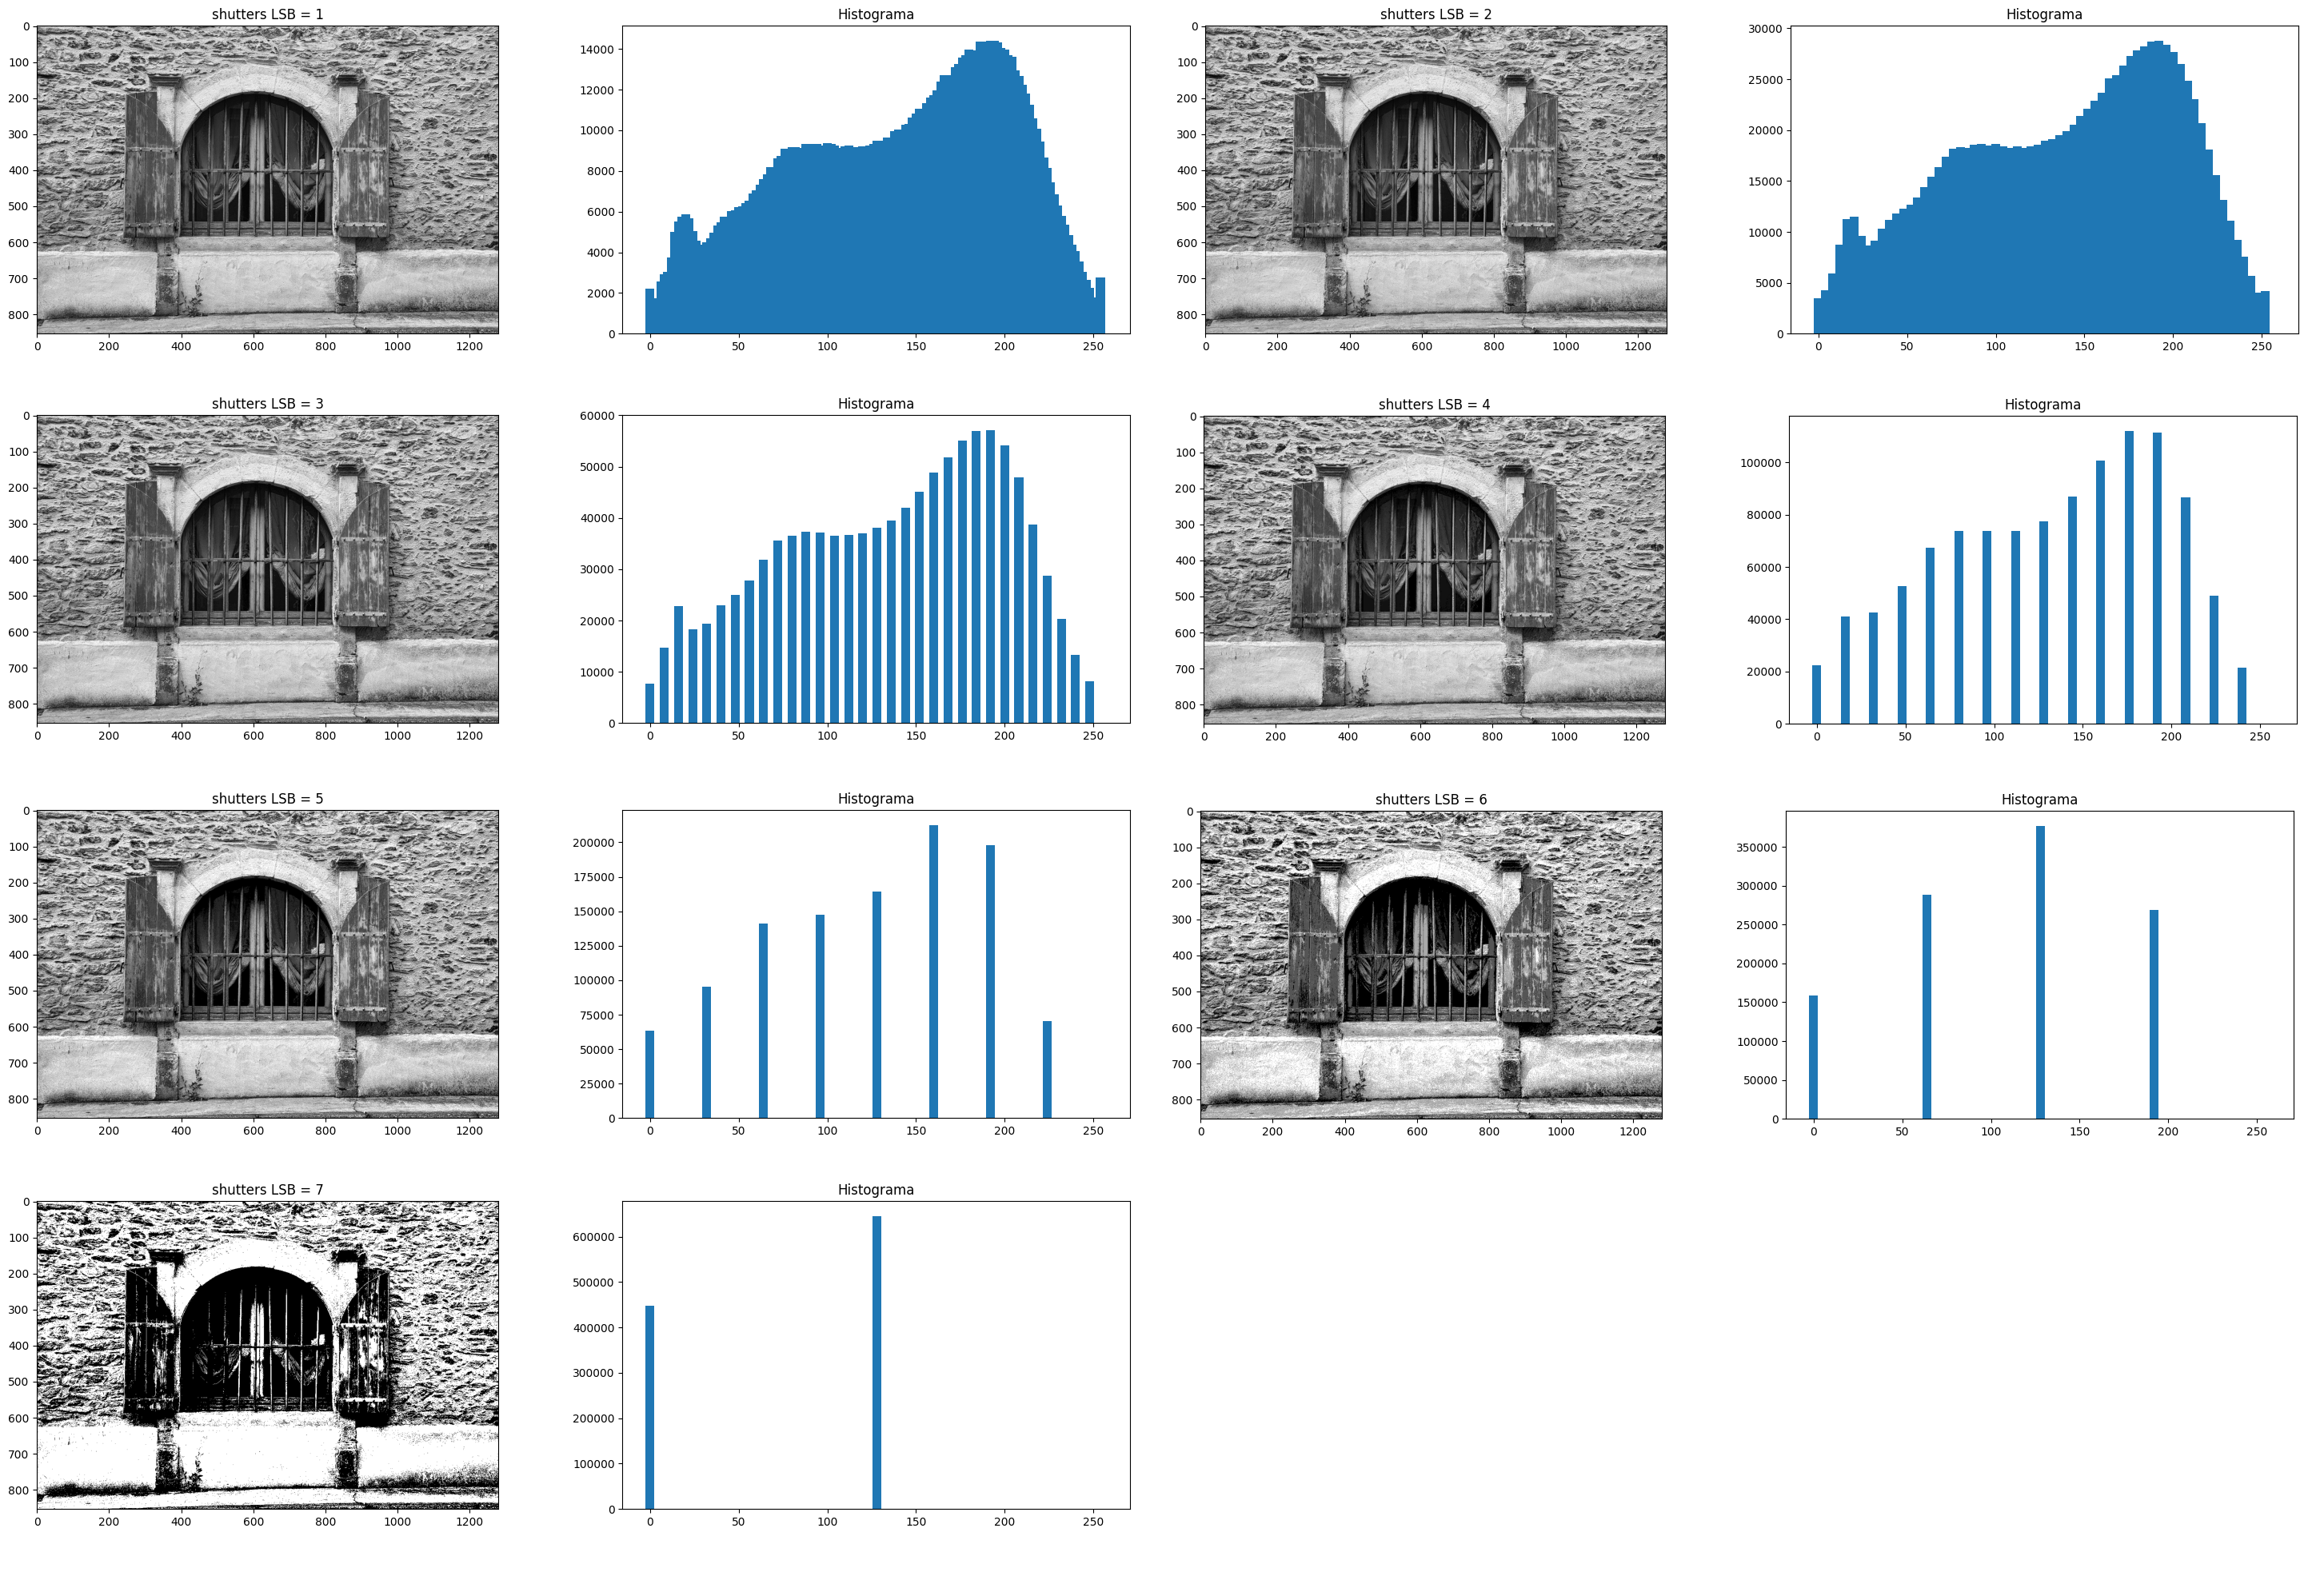
\includegraphics[width=1\linewidth]{Elementos//Figuras/shutters_lsb.png}
    \caption{Da esquerda para a direita e de cima para baixo temos: Imagem Shutters com 1, 2, 3, 4, 5, 6 e 7 LSBs zerados.}
    \label{fig:shutters-lsb}
\end{figure}

\begin{figure}[h!]
    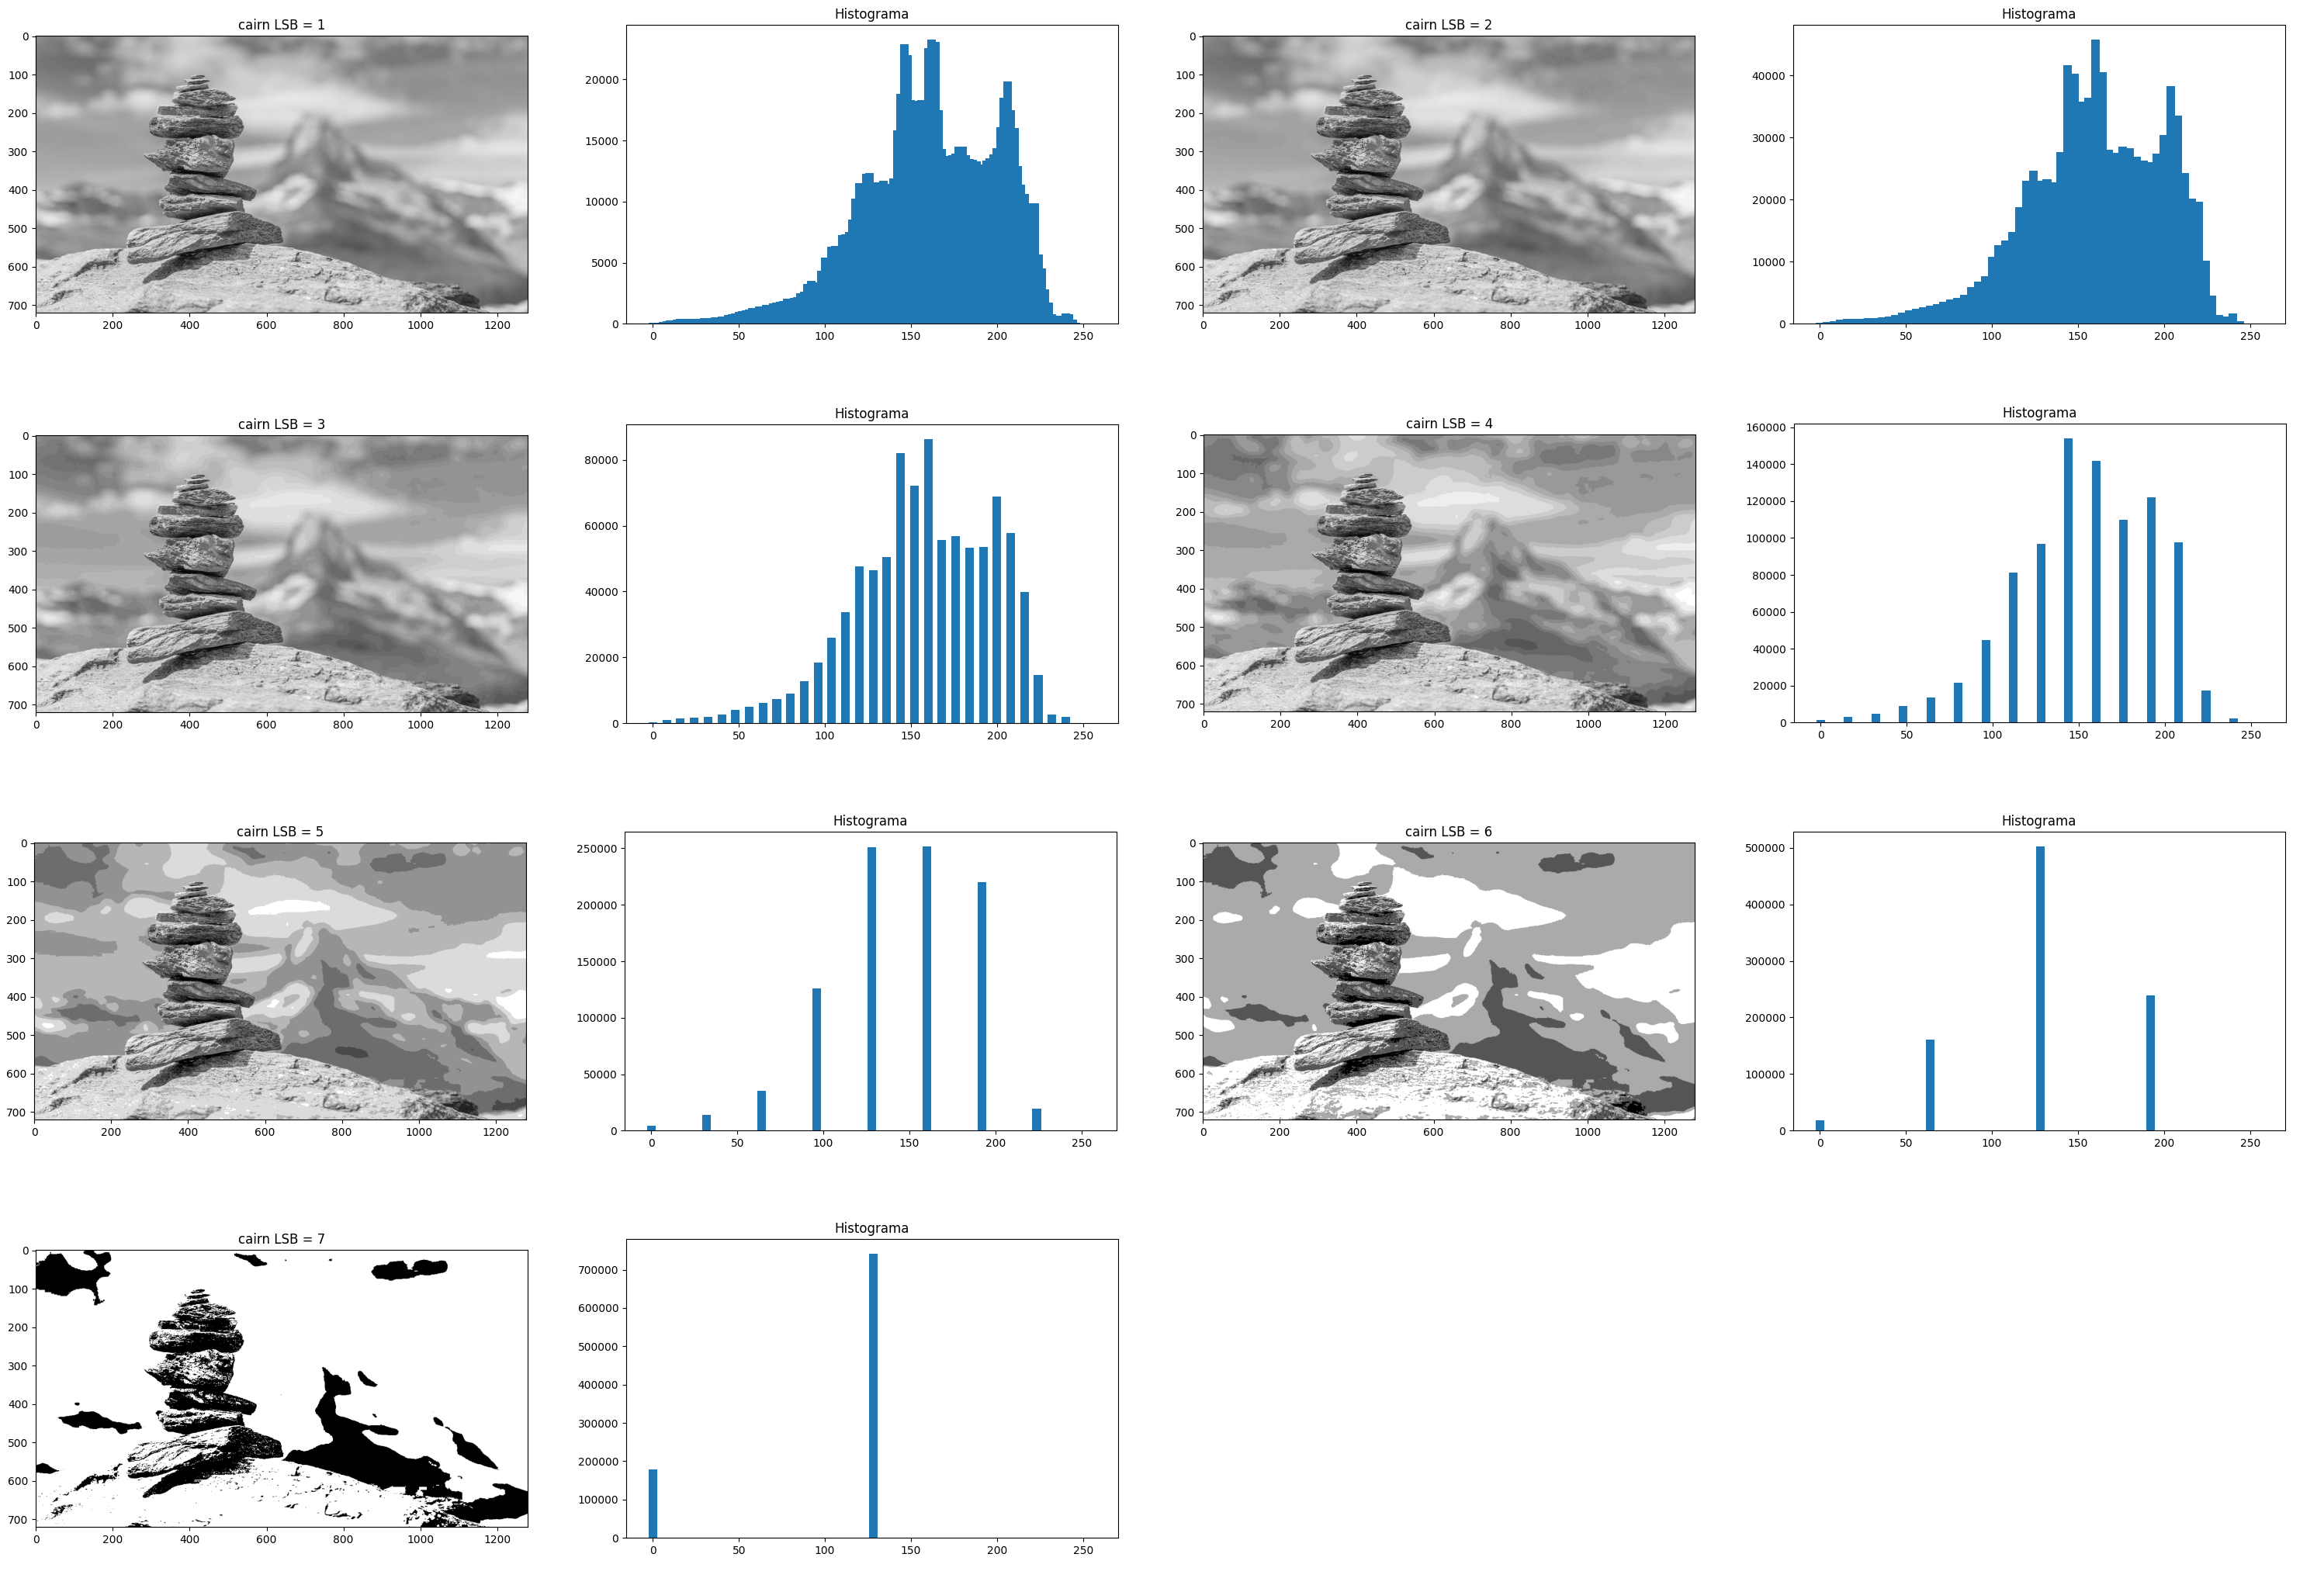
\includegraphics[width=1\linewidth]{Elementos//Figuras/cairn_lsb.png}
    \caption{Da esquerda para a direita e de cima para baixo temos: Imagem Cairn com 1, 2, 3, 4, 5, 6 e 7 LSBs zerados.}
    \label{fig:cairn-lsb}
\end{figure}

Ao realizar uma análise subjetiva das imagens modificadas, percebe-se que todas as imagens, com exceção da imagem \textit{shutters} (Figura \ref{fig:shutters-lsb}), não apresentam ruídos visualmente perceptíveis quando se utiliza até 4 LSBs para ocultação de informações. A imagem \textit{shutters}, por sua vez, não apresenta grandes distorções utilizando até 5 LSBs.

% ---------------------------------------------------------------- %

\subsection{Comparação dos histogramas das imagens com MSBs zerados}

Semelhante ao que foi feito nos experimentos com os LSBs, as imagens com 1, 2, 3, 4, 5, 6 e 7 MSBs (Figuras \ref{fig:swan-msb} a \ref{fig:cairn-msb}) foram dispostas lado a lado. Ao lado de cada imagem está o seu histograma, por meio do qual pode-se observar a diminuição do número de tonalidades conforme a quantidade de MSBs aumenta. 

\begin{figure}[h!]
    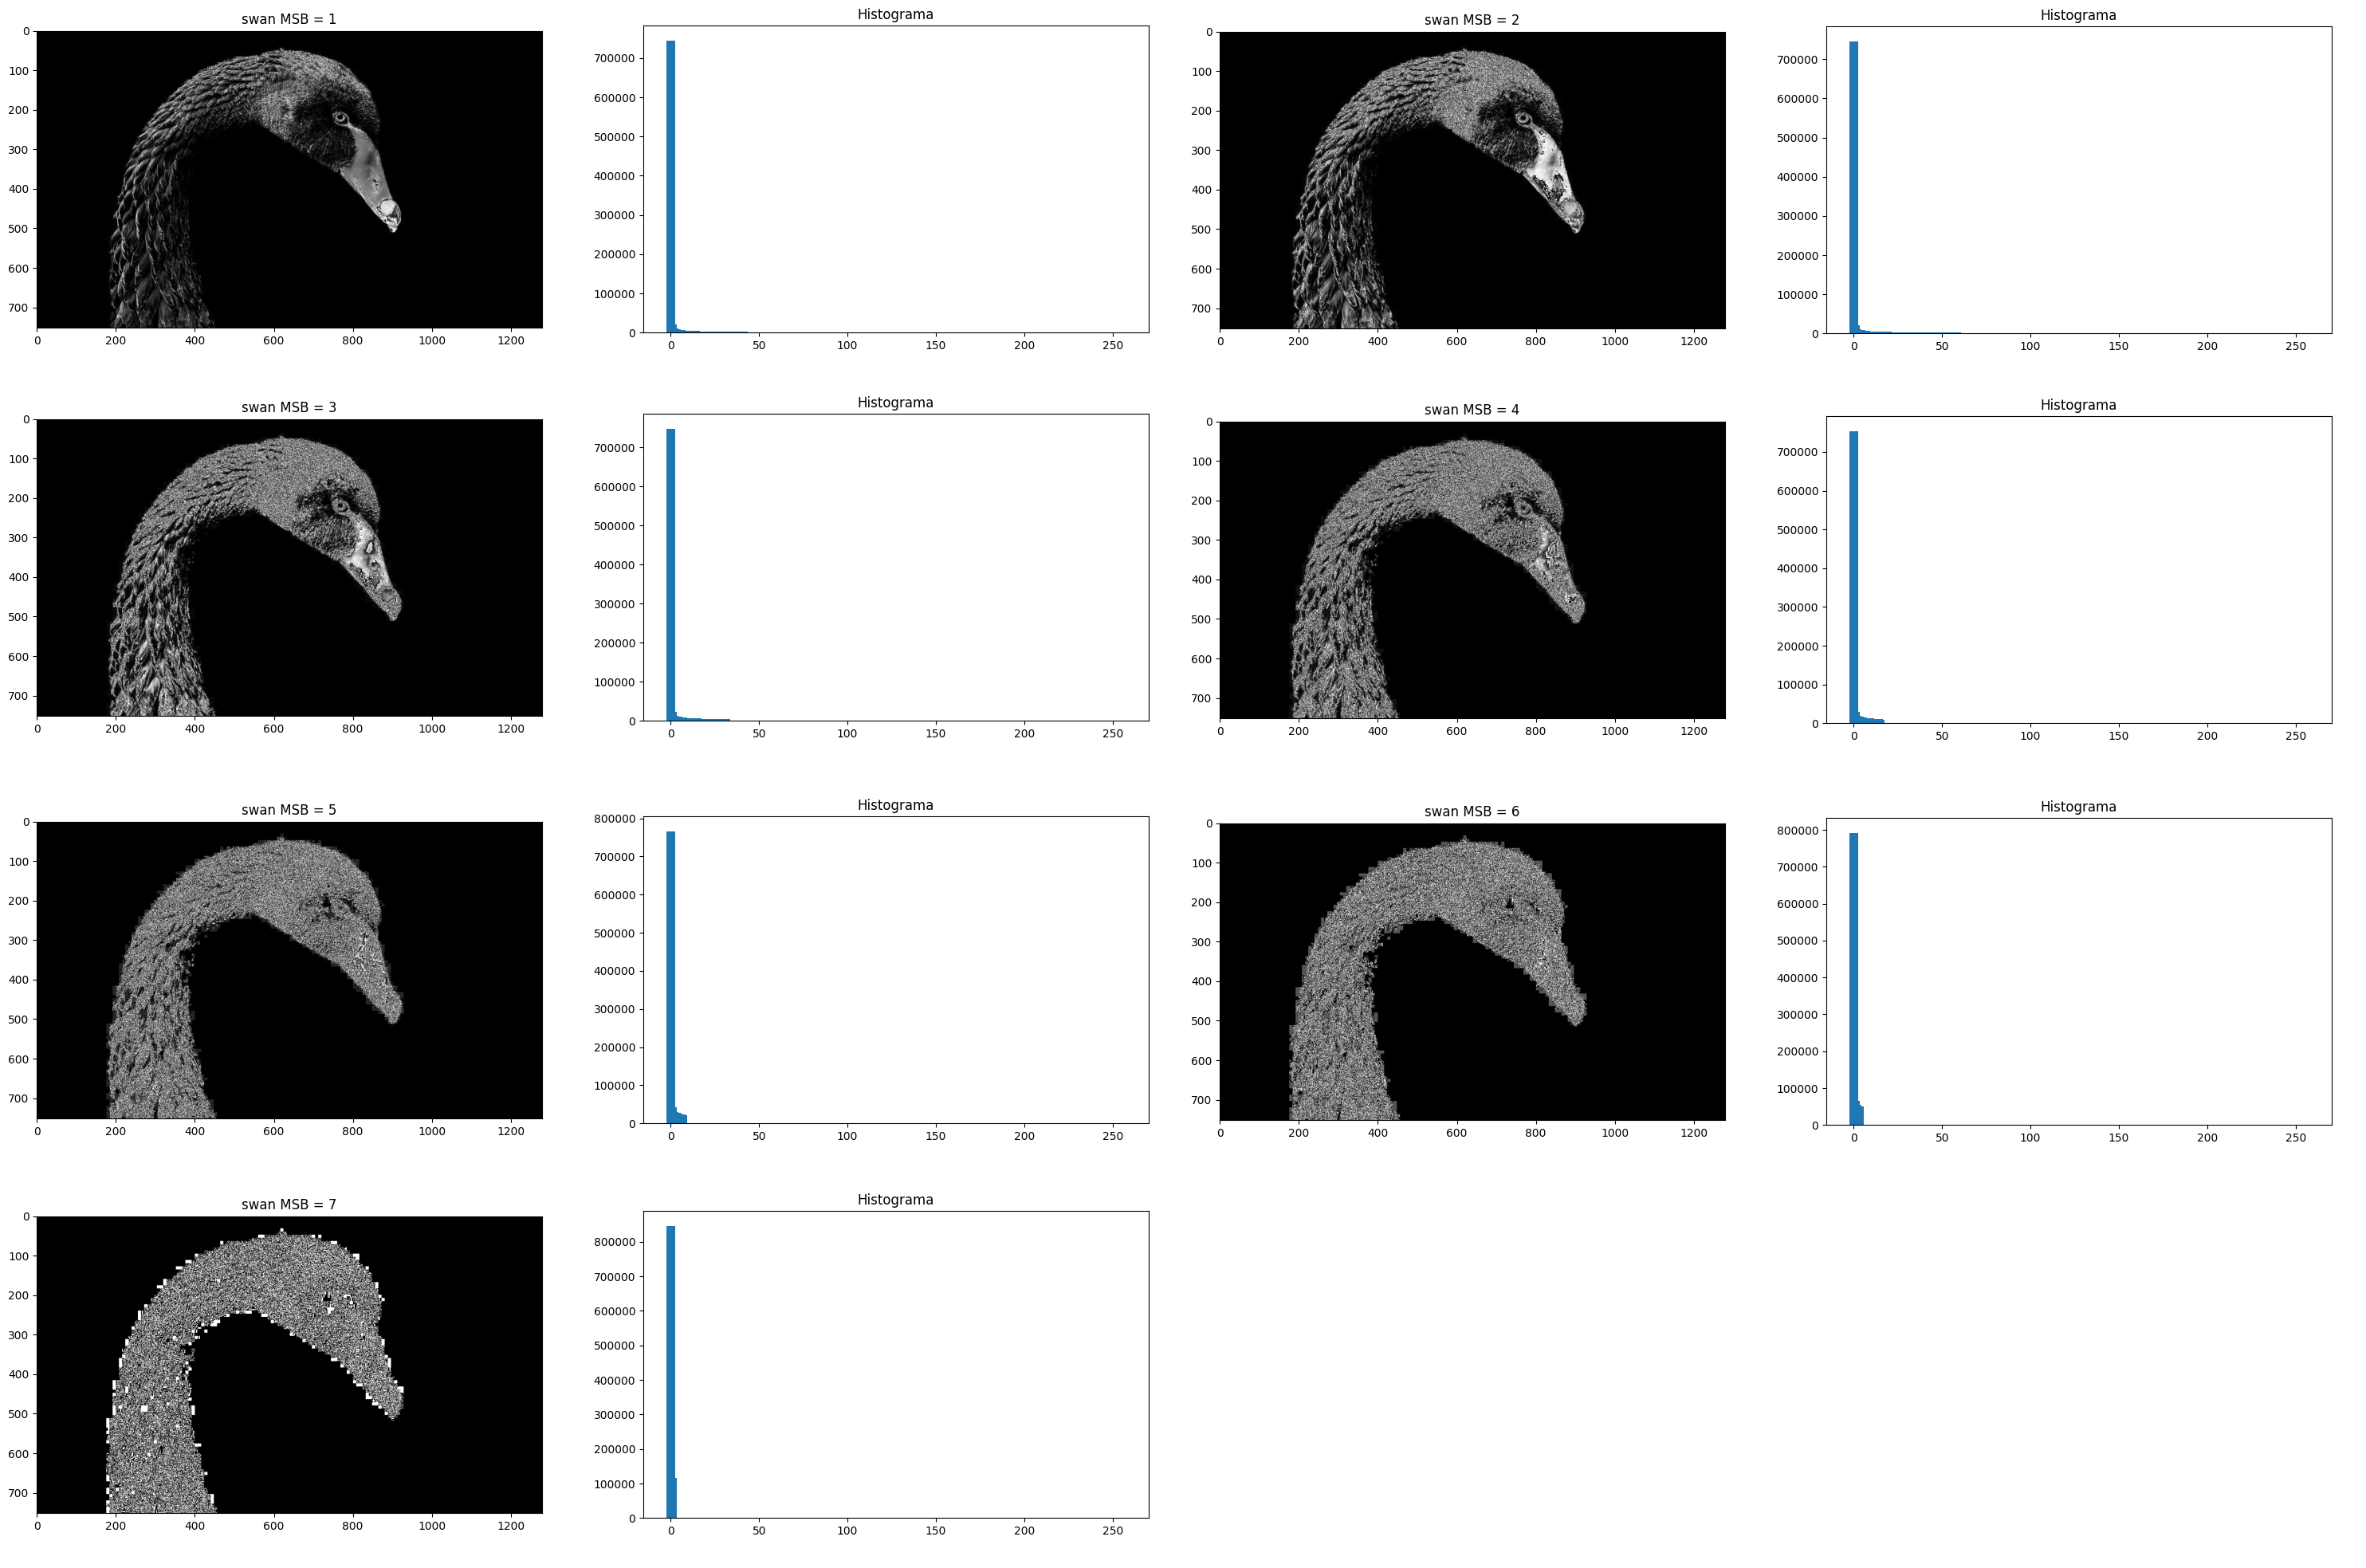
\includegraphics[width=1\linewidth]{Elementos//Figuras/swan_msb.png}
    \caption{Da esquerda para a direita e de cima para baixo temos: Imagem Swan com 1, 2, 3, 4, 5, 6 e 7 MSBs zerados.}
    \label{fig:swan-msb}
\end{figure}

\begin{figure}[h!]
    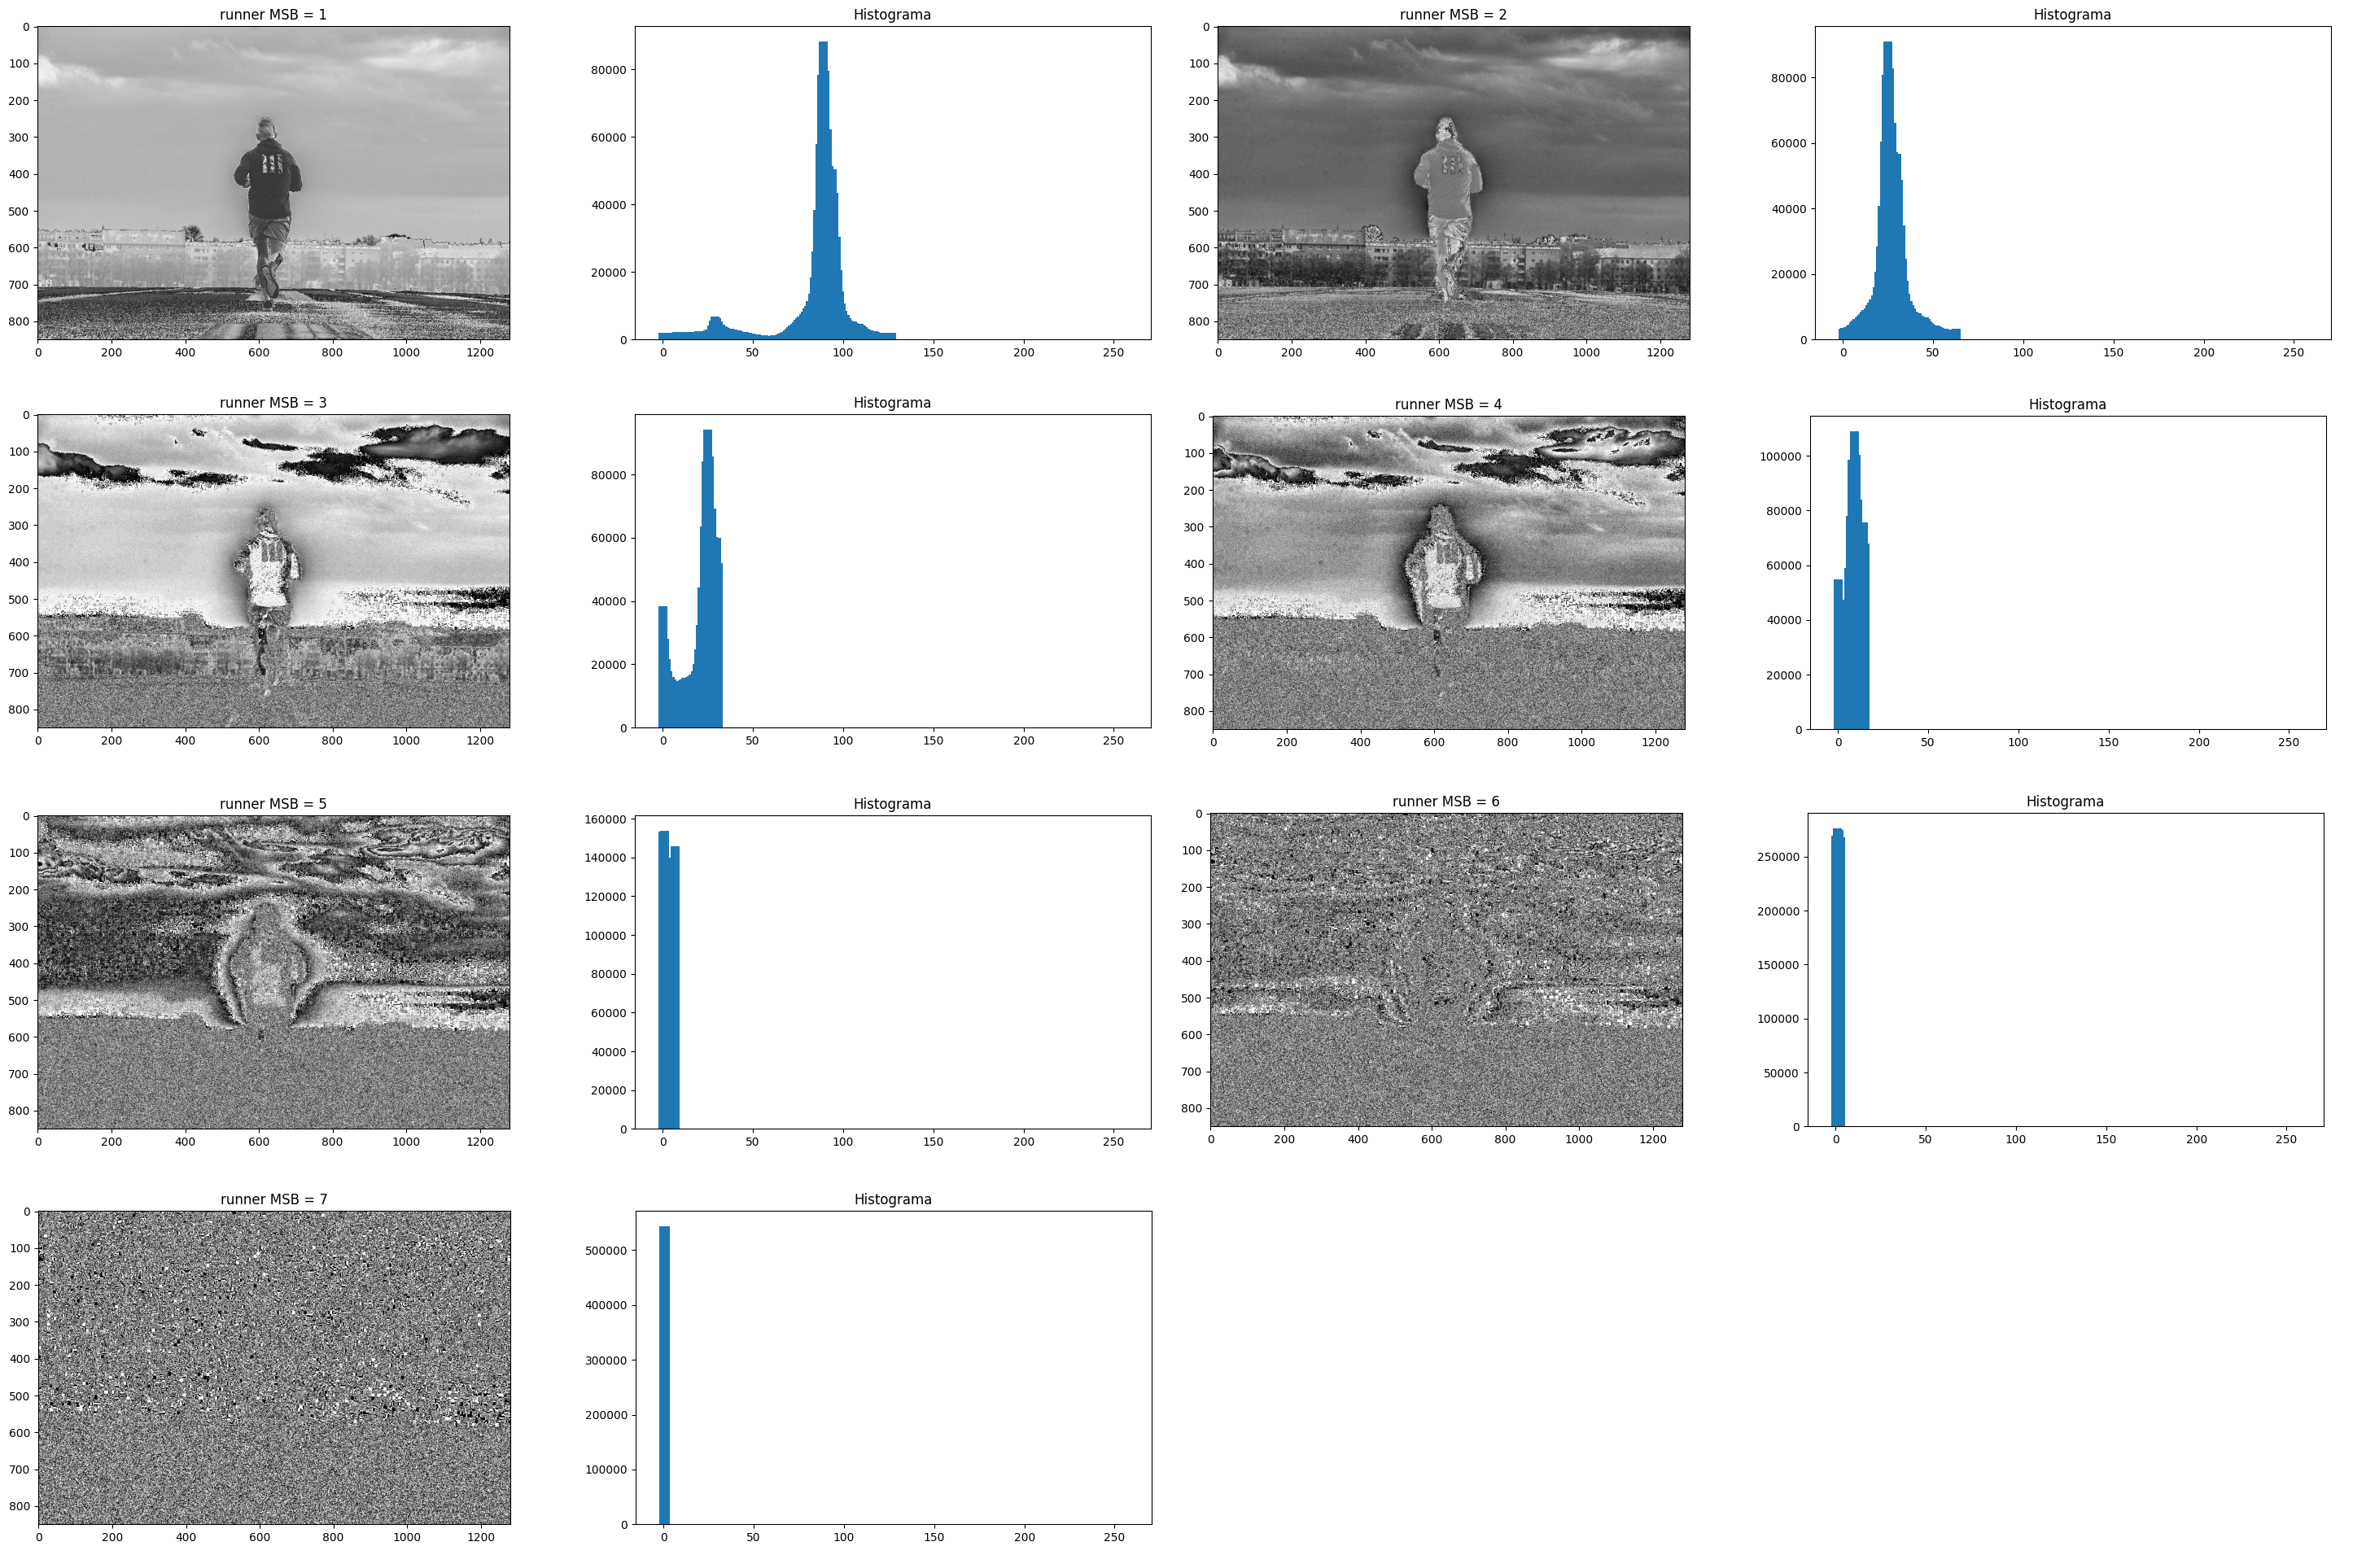
\includegraphics[width=1\linewidth]{Elementos//Figuras/runner_msb.png}
    \caption{Da esquerda para a direita e de cima para baixo temos: Imagem Runner com 1, 2, 3, 4, 5, 6 e 7 MSBs zerados.}
    \label{fig:runner-msb}
\end{figure}

\begin{figure}[h!]
    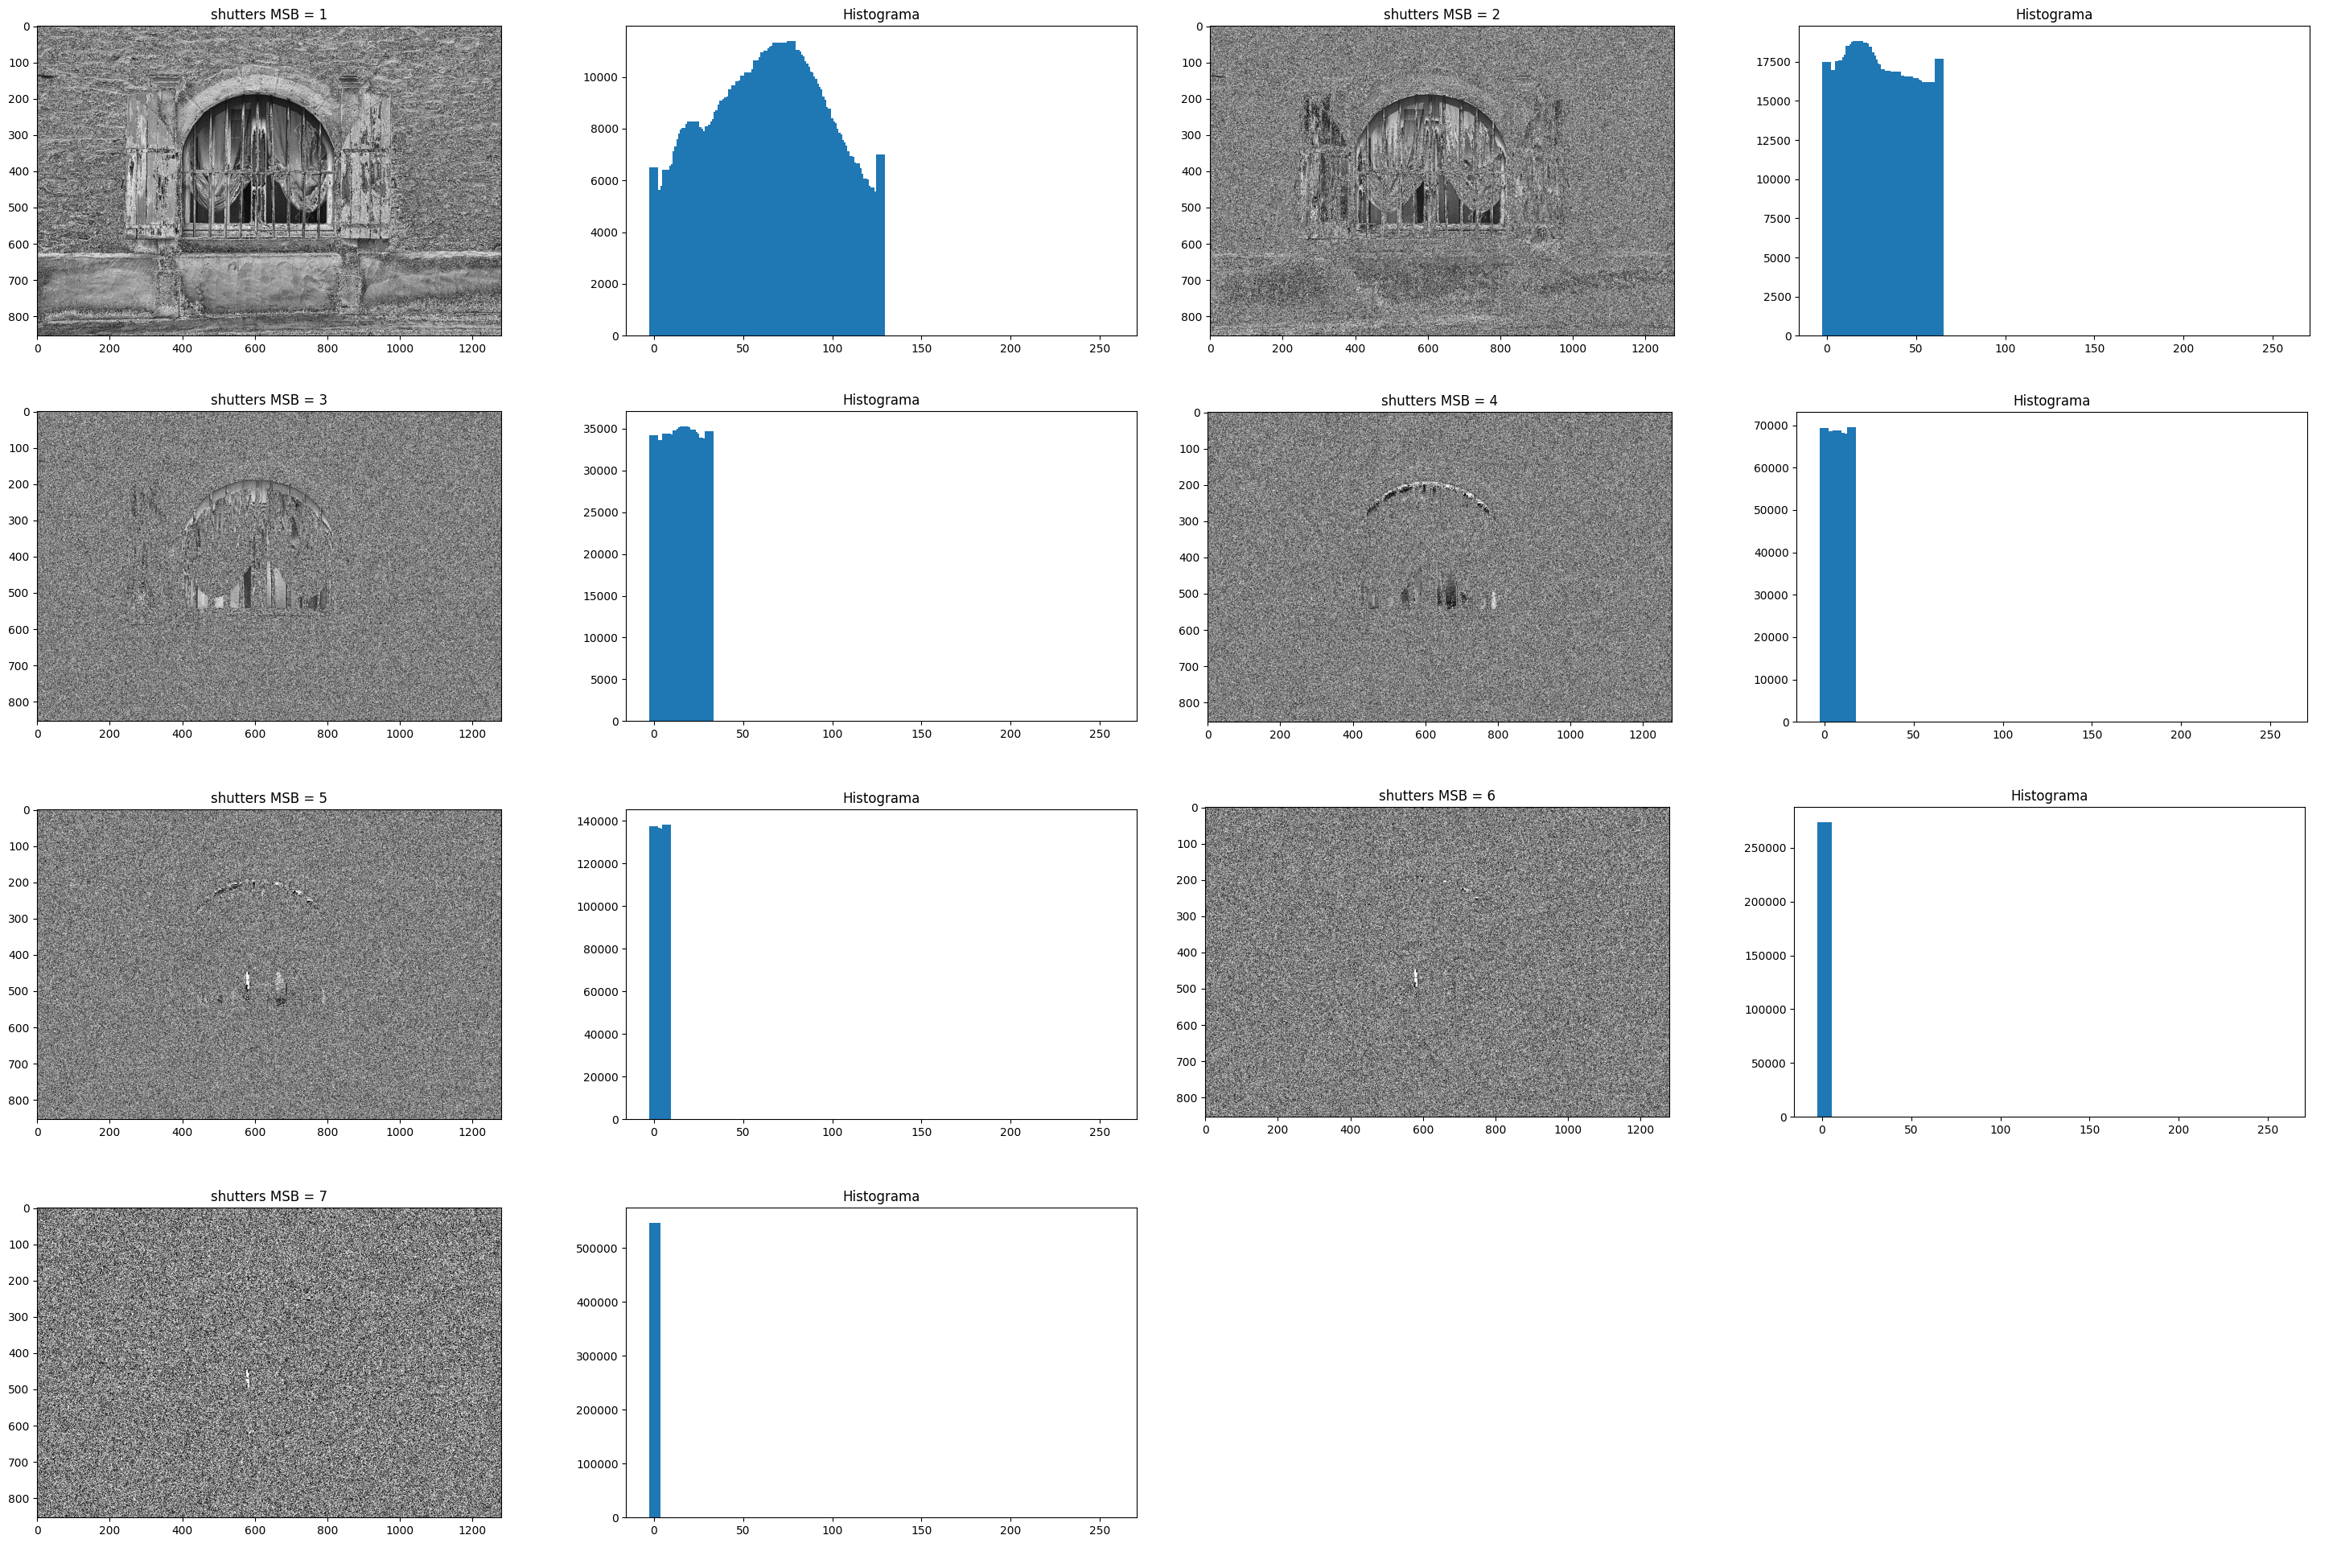
\includegraphics[width=1\linewidth]{Elementos//Figuras/shutters_msb.png}
    \caption{Da esquerda para a direita e de cima para baixo temos: Imagem Shutters com 1, 2, 3, 4, 5, 6 e 7 MSBs zerados.}
    \label{fig:shutters-msb}
\end{figure}

\begin{figure}[h!]
    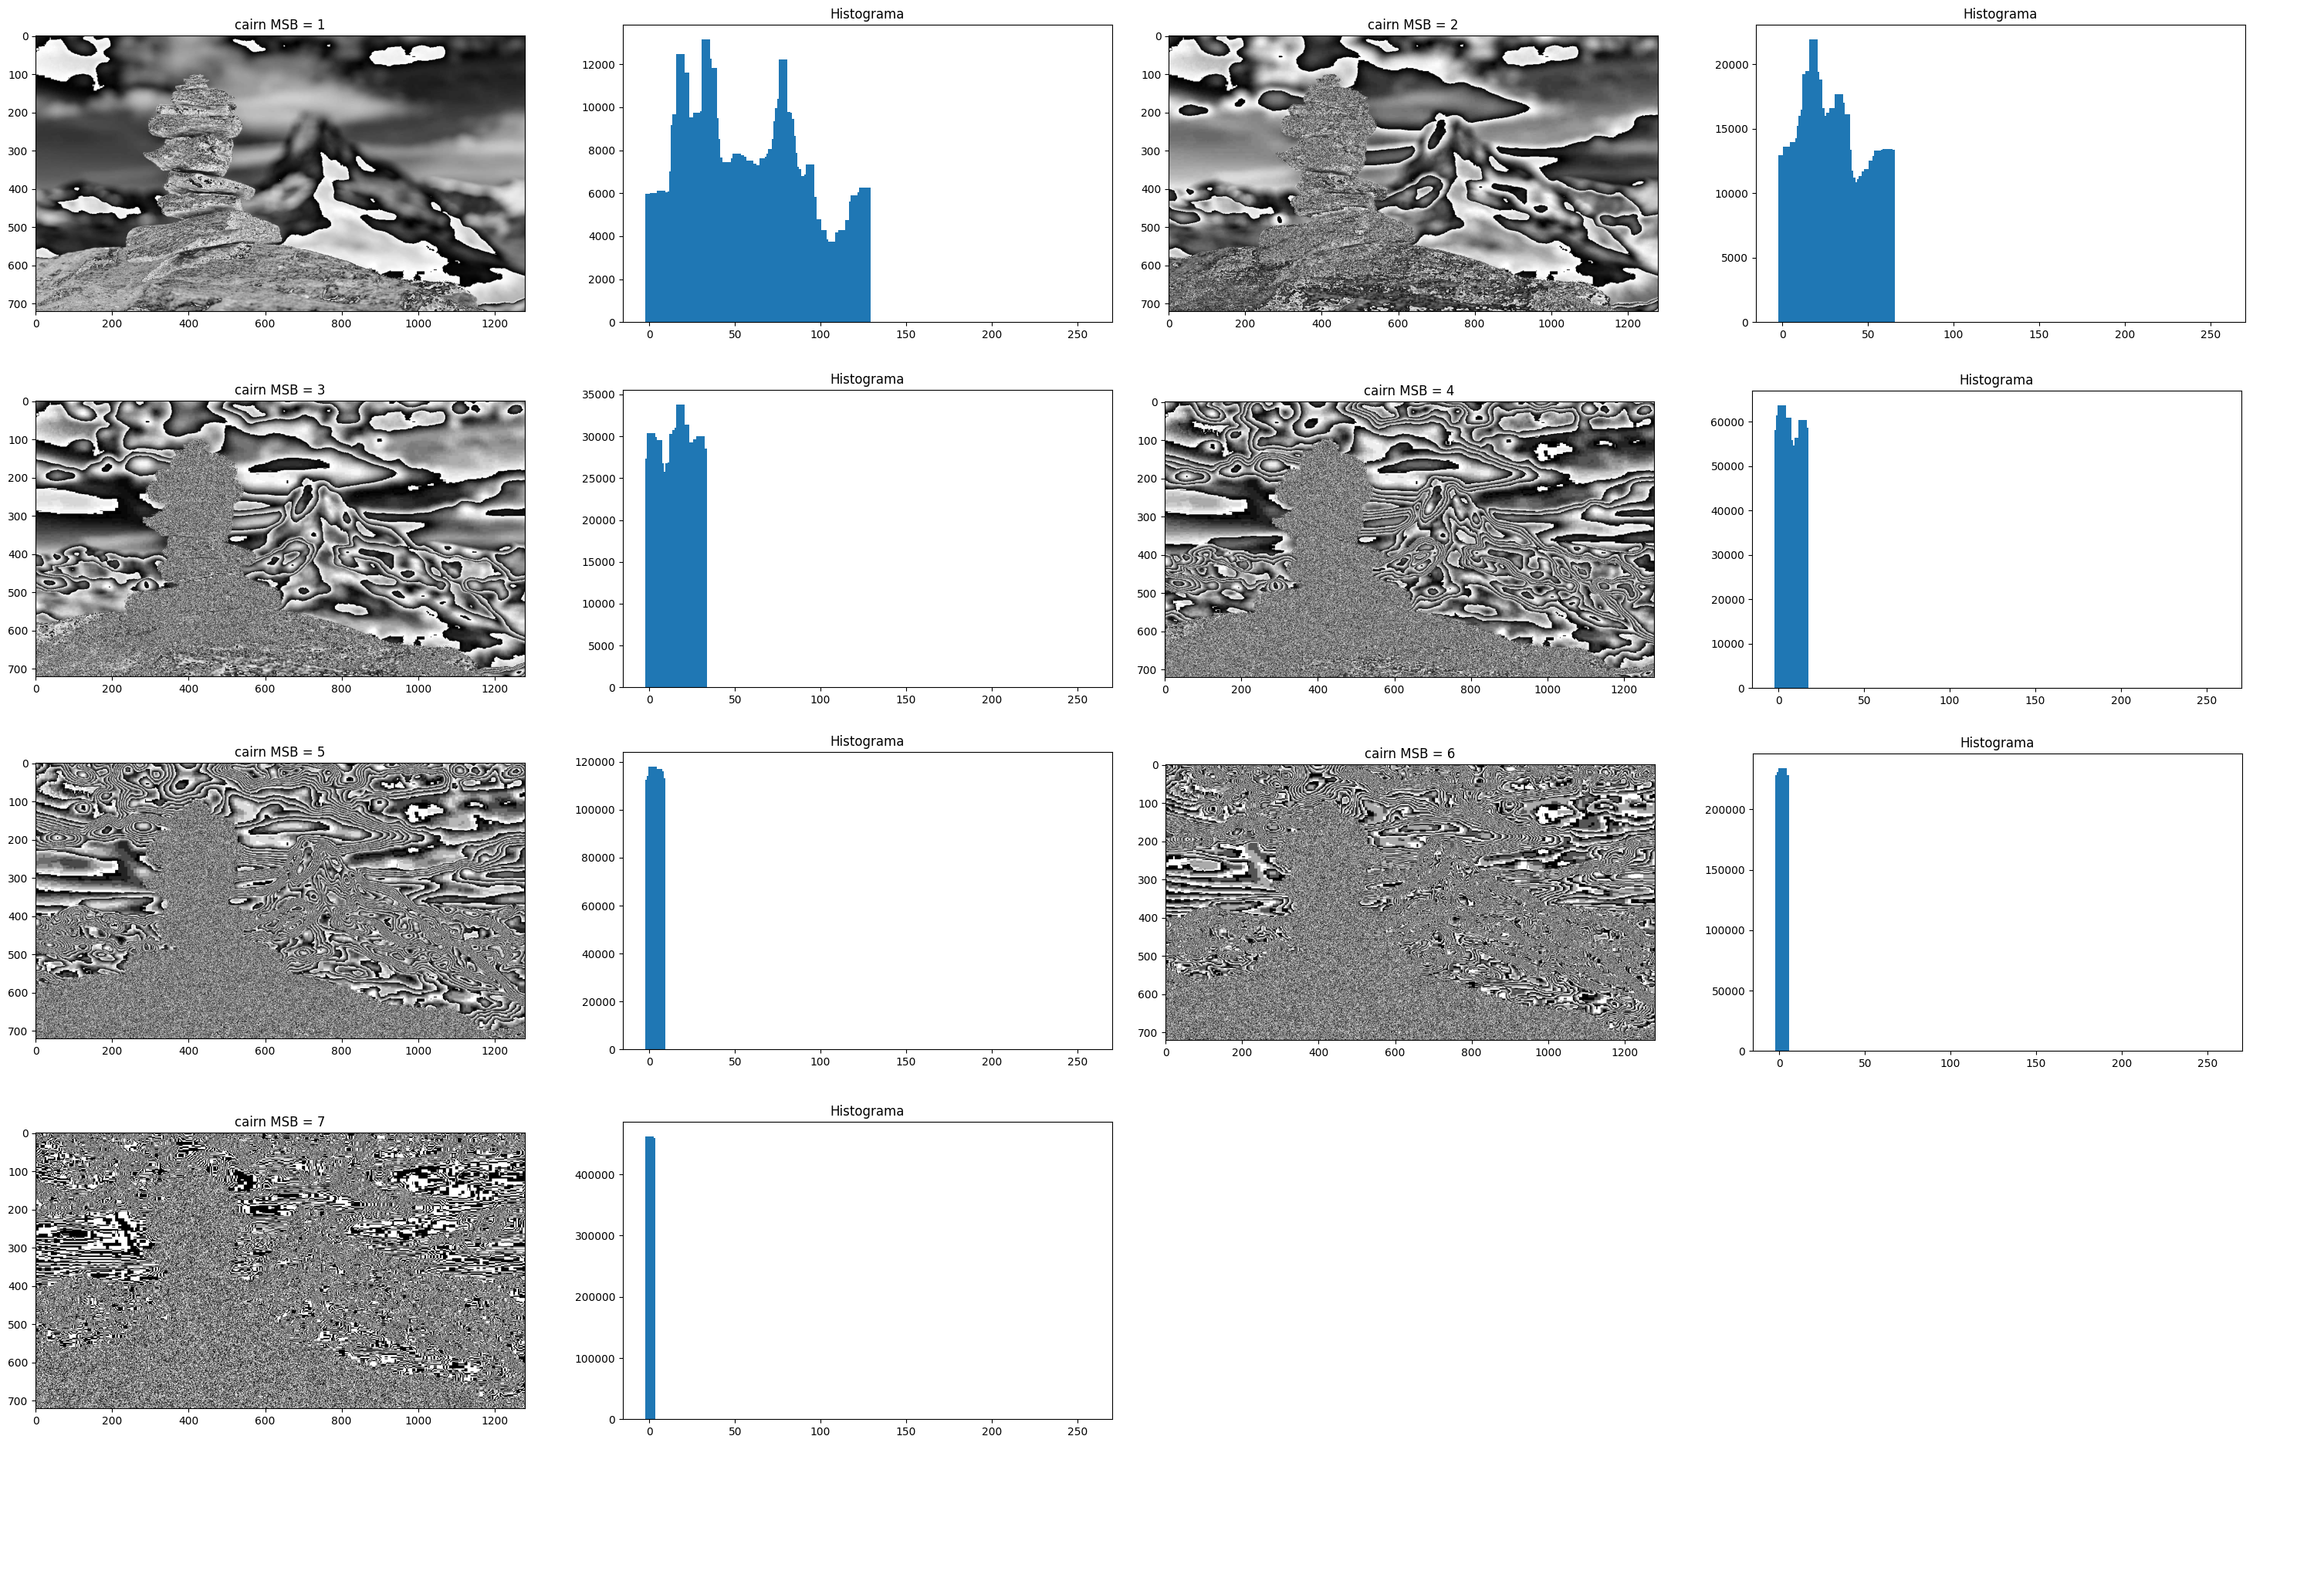
\includegraphics[width=1\linewidth]{Elementos//Figuras/cairn_msb.png}
        \caption{Da esquerda para a direita e de cima para baixo temos: Imagem Cairn com 1, 2, 3, 4, 5, 6 e 7 MSBs zerados.}
    \label{fig:cairn-msb}
\end{figure}

Percebe-se que a quantidade de ruídos apresentada é muito maior mesmo quando apenas um MSB é zerado. Isso ocorre porque, diferentemente dos LSBs, os MSBs têm grande influência sobre a informação. Dessa forma, quando o \textit{bit} mais significativo de um \textit{pixel} foi zerado, a quantidade de tonalidades possíveis para aquele \textit{pixel}, caiu pela metade.

\subsection{Análise das métricas objetivas das imagens com LSBs e MSBs zerados}

A Tabela \ref{tab:resultados-psnr-ssim} permite, por meio das métricas objetivas PSNR e SSIM, a análise da quantidade máxima de LSBs e MSBs que podem ser utilizados para ocultar informações em cada imagem. Todas as imagens que utilizaram até quatro LSBs apresentaram um SSIM acima de $0.9$, o que indica um nível alto de semelhança com a imagem original.

\begin{table}
\begin{tabular}{ccccccccc}
\hline
& \multicolumn{2}{c}{cairn} & \multicolumn{2}{c}{runner} & \multicolumn{2}{c}{shutters} & \multicolumn{2}{c}{swan} \\
& PSNR & SSIM & PSNR & SSIM & PSNR & SSIM & PSNR & SSIM \\
\hline
LSB 1 & 51.1575 & 0.9974 & 51.1388 & 0.9971 & 51.1370 & 0.9997 & 57.3143 & 0.9985 \\
LSB 2 & 42.6962 & 0.9881 & 42.7157 & 0.9862 & 42.6864 & 0.9985 & 49.3048 & 0.9943 \\
LSB 3 & 35.6999 & 0.9601 & 35.7731 & 0.9508 & 35.6897 & 0.9935 & 42.6692 & 0.9811 \\
LSB 4 & 29.3002 & 0.9016 & 28.6152 & 0.9076 & 29.2425 & 0.9745 & 36.6770 & 0.9489 \\
LSB 5 & 22.9212 & 0.8368 & 21.1971 & 0.7985 & 23.0121 & 0.9097 & 30.9843 & 0.8891 \\
LSB 6 & 17.2683 & 0.7523 & 18.8059 & 0.7843 & 17.0194 & 0.7504 & 25.9452 & 0.8202 \\
LSB 7 & 11.5796 & 0.5277 & 9.4766 & 0.5577 & 11.0111 & 0.3688 & 22.6162 & 0.7695 \\
\hline
MSB 1 & 6.9259 & 0.4390 & 7.1952 & 0.6076 & 8.2724 & 0.2938 & 28.5954 & 0.9780 \\
MSB 2 & 5.2902 & 0.2337 & 3.8795 & 0.2474 & 6.1461 & 0.0507 & 24.5492 & 0.9166 \\
MSB 3 & 4.5613 & 0.1089 & 3.5696 & 0.1169 & 5.2922 & 0.0205 & 22.8298 & 0.8587 \\
MSB 4 & 4.1211 & 0.0347 & 2.9918 & 0.0351 & 4.8618 & 0.0030 & 21.9574 & 0.8102 \\
MSB 5 & 3.9201 & 0.0099 & 2.7581 & 0.0037 & 4.6506 & 0.0003 & 21.5006 & 0.7812 \\
MSB 6 & 3.8171 & 0.0018 & 2.6761 & 0.0007 & 4.5456 & 0.0000 & 21.2674 & 0.7628 \\
MSB 7 & 3.7659 & 0.0001 & 2.6324 & 0.0000 & 4.4935 & 0.0000 & 21.1479 & 0.7510 \\
\hline
\end{tabular}
\caption{Tabela com as métricas PSNR e SSIM após modificação de \textit{bits} menos e mais significativos}
\label{tab:resultados-psnr-ssim}
\end{table}

Somente a imagem \textit{swan} com 1 e 2 MSBs (Figura \ref{fig:swan-msb}) presentou um SSIM acima $0.9$ quando os MSBs foram zerados. Isso ocorre devido ao fato de que a imagem \textit{swan} original é rica em tons escuros. Os tons escuros são representados por valores próximos a zero, o que faz com que o \textit{bit} mais significativo dos \textit{pixels} mais escuros já seja zero.